% Versão 24/06/2020

% Este documento destina-se a servir como modelo para a produção de documentos
% de pesquisa do PPGINF/UFPR, como projetos, dissertações e teses. A classe de
% documento se chama "ppginf" (arquivo ppginf.cls) e define o formato básico do
% documento. O texto está organizado em capítulos que são colocados em
% subdiretórios separados. São definidos exemplos para a inclusão de figuras,
% códigos-fonte e a definição de tabelas.
%
% Produzido por Carlos Maziero (maziero@inf.ufpr.br).

%=====================================================

% Opções da classe ppginf:
%
% - defesa    : versão para entregar à banca; tem espaçamento 1,5
%               e omite algumas páginas iniciais (agradecimentos, etc)
% - final     : versão pós-defesa, para enviar à biblioteca;
%               tem espaçamento simples e todas as páginas iniciais.
% - oneside   : somente frente; use quando for gerar somente o PDF.
% - twoside   : frente/verso; use se precisar de uma versão impressa.
% - metadados : inclui metadados no PDF (por default não inclui)
% - ...       : demais opções aceitas pela classe "book"

% ATENÇÂO: este modelo tem suporte para português e inglês.
% As duas línguas devem ser informadas como opção da classe;
% a língua principal do documento deve vir POR ÚLTIMO.

% Versão de defesa em português
\documentclass[defesa,oneside,english,brazilian]{ppginf}

% Versão de defesa em inglês
%\documentclass[defesa,oneside,brazilian,english]{ppginf}

% Versão final em PDF para a biblioteca da UFPR (português e inglês)
%\documentclass[final,oneside,english,brazilian]{ppginf}
%\documentclass[final,oneside,brazilian,english]{ppginf}

% Versão final para impressão (frente/verso)
%\documentclass[final,twoside,english,brazilian]{ppginf}

% configurações de diversos pacotes, inclusive a fonte usada no texto
% Pacotes usados neste documento e suas respectivas configurações

% ------------------------------------------------------------------------------

% Definição de fontes

% formato dos arquivos-fonte (utf8 no Linux e latin1 no Windows)
\usepackage[utf8]{inputenc}	% arquivos LaTeX em Unicode (UTF8)

% usar codificação T1 para ter caracteres acentuados corretos no PDF
\usepackage[T1]{fontenc}

% fonte usada no corpo do texto (pode alterar, mas descomente apenas uma)
\usepackage{newtxtext,newtxmath}	% Times (se não tiver, use mathptmx)
%\usepackage{lmodern}			% Computer Modern (fonte clássico LaTeX)
%\usepackage{kpfonts}			% Kepler/Palatino (idem, use mathpazo)
%\renewcommand{\familydefault}{\sfdefault} % Arial/Helvética (leia abaixo)

% A biblioteca central da UFPR recomenda usar Arial, seguindo a recomendação da
% ABNT. Essa é uma escolha ruim, pois fontes sans-serif são geralmente inade-
% quados para textos longos e impressos, sendo melhores para páginas Web.
% http://www.webdesignerdepot.com/2013/03/serif-vs-sans-the-final-battle/.

% fontes usadas em ambientes específicos
\usepackage[scaled=0.9]{helvet}		% Sans Serif
\usepackage{courier}			% Verbatim, Listings, etc

% ------------------------------------------------------------------------------

% inclusão de figuras em PDF, PNG, PS, EPS
\usepackage{graphicx}

% subfiguras (subfigure is deprecated, don't use it)
\usepackage[labelformat=simple]{subcaption}
\renewcommand\thesubfigure{(\alph{subfigure})}

% ------------------------------------------------------------------------------

% inclusão/formatação de código-fonte (programas)
\usepackage{listings}
\lstset{language=c}
\lstset{basicstyle=\ttfamily\footnotesize,commentstyle=\textit,stringstyle=\ttfamily}
\lstset{showspaces=false,showtabs=false,showstringspaces=false}
\lstset{numbers=left,stepnumber=1,numberstyle=\tiny}
\lstset{columns=flexible,mathescape=true}
\lstset{frame=single}
\lstset{inputencoding=utf8,extendedchars=true}
\lstset{literate={á}{{\'a}}1  {ã}{{\~a}}1 {à}{{\`a}}1 {â}{{\^a}}1
                 {Á}{{\'A}}1  {Ã}{{\~A}}1 {À}{{\`A}}1 {Â}{{\^A}}1
                 {é}{{\'e}}1  {ê}{{\^e}}1 {É}{{\'E}}1  {Ê}{{\^E}}1
                 {í}{{\'\i}}1 {Í}{{\'I}}1
                 {ó}{{\'o}}1  {õ}{{\~o}}1 {ô}{{\^o}}1
                 {Ó}{{\'O}}1  {Õ}{{\~O}}1 {Ô}{{\^O}}1
                 {ú}{{\'u}}1  {Ú}{{\'U}}1
                 {ç}{{\c{c}}}1 {Ç}{{\c{C}}}1 }

% ------------------------------------------------------------------------------

% formatação de algoritmos
\usepackage{algorithm,algorithmic}
\IfLanguageName{brazilian} {\floatname{algorithm}{Algoritmo}}{}
\renewcommand{\algorithmiccomment}[1]{~~~// #1}
%\algsetup{linenosize=\footnotesize,linenodelimiter=.}

% ------------------------------------------------------------------------------

% formatação de bibliografia
\usepackage{natbib}			% bibliografia no estilo NatBib
\IfLanguageName{brazilian}
{\bibliographystyle{apalike-ptbr}}	% formato em português
{\bibliographystyle{apalike}}		% formato em inglês

% Estilos de bibliografia recomendados (só descomentar um estilo!)
% Mais infos: https://pt.sharelatex.com/learn/Bibtex_bibliography_styles
%
%\bibliographystyle{apalike-ptbr}	% [Maziero et al., 2006]
%\bibliographystyle{alpha}		% [Maz06]
%\bibliographystyle{plainnat}		% vide Google "LaTeX Natbib"
%\bibliographystyle{plain}		% [1] ordem alfabética
%\bibliographystyle{unsrt}		% [1] ordem de uso no texto

% no estilo "unsrt", evita que citações nos índices sejam consideradas
%\usepackage{notoccite}

\renewcommand{\cite}{\citep}	% \cite deve funcionar como \citep
%\bibpunct{[}{]}{;}{a}{}{,}	% caracteres usados nas referências

% ------------------------------------------------------------------------------

% fontes adicionais
\usepackage{amsmath}		% pacotes matemáticos
\usepackage{amsfonts}		% fontes matemáticas 
%\usepackage{amssymb}		% símbolos 

% ------------------------------------------------------------------------------

% pacotes diversos
\usepackage{alltt,moreverb}	% mais comandos no modo verbatim
\usepackage{lipsum}		% gera texto aleatório (para os exemplos)
\usepackage{currfile}		% infos sobre o arquivo/diretório atual
\usepackage[final]{pdfpages}	% inclusão de páginas em PDF
\usepackage{longtable}		% tabelas multi-páginas (tab símbolos/acrônimos)

% ------------------------------------------------------------------------------

% \usepackage{amsthm}
\newtheorem{definition}{Definição}


%=====================================================

\begin {document}

% Principais dados, usados para gerar as páginas iniciais.
% Campos não utilizados podem ser removidos ou comentados.

% título
\title{Explorando propriedades da centralidade de caminhos mínimos em grafos complexos.}

% palavras-chave e keywords (p/ resumo, abstract e metadados do PDF)
\pchave{Teoria dos grafos. Caminhos mínimos. Grafos complexos. Algoritmo de Dijkstra.}
% \keyword{Keyword 1. Keyword 2. Keyword 3.}

% autoria
\author{Ricardo Norio Miyata}
\advisor{Murilo V. G. da Silva}
% \coadvisor{Leslie Lamport}

% instituição
\IfLanguageName{brazilian}
  { \instit{UFPR}{Universidade Federal do Paraná} }
% a Bib/UFPR exige que tudo seja em português, exceto o título :-(
%  { \instit{UFPR}{Federal University of Paraná} }
  { \instit{UFPR}{Universidade Federal do Paraná} }

% área de concentração (default do PPGInf, não mudar)
\IfLanguageName{brazilian}
  { \field{Ciência da Computação} }
% a Bib/UFPR exige que tudo seja em português, exceto o título :-(
%  { \field{Computer Science} }
  { \field{Ciência da Computação} }

% data (só o ano)
\date{2021}

% local
\IfLanguageName{brazilian}
  { \local{Curitiba PR} }
% a Bib/UFPR exige que tudo seja em português, exceto o título :-(
%  { \local{Curitiba PR - Brazil} }
  { \local{Curitiba PR} }

% imagem de fundo da capa (se não desejar, basta comentar)
\coverimage{0-iniciais/fundo-capa.jpg}

%=====================================================

%% Descrição do documento (obviamente, descomentar somente UMA!)

% Por exigência da biblioteca da UFPR, a descrição do documento deve ser
% em português, mesmo em documentos em outras línguas. Vá entender...

% tese de doutorado
% \descr{Tese apresentada como requisito parcial à obtenção do grau de Doutor em Ciência da Computação no Programa de Pós-Graduação em Informática, Setor de Ciências Exatas, da Universidade Federal do Paraná}

% exame de qualificação de doutorado
%\descr{Documento apresentado como requisito parcial ao exame de qualificação de Doutorado no Programa de Pós-Graduação em Informática, Setor de Ciências Exatas, da Universidade Federal do Paraná}

% dissertação de mestrado
%\descr{Dissertação apresentada como requisito parcial à obtenção do grau de Mestre em Informática no Programa de Pós-Graduação em Informática, Setor de Ciências Exatas, da Universidade Federal do Paraná}

% exame de qualificação de mestrado
%\descr{Documento apresentado como requisito parcial ao exame de qualificação de Mestrado no Programa de Pós-Graduação em Informática, Setor de Ciências Exatas, da Universidade Federal do Paraná}

% trabalho de conclusão de curso
\descr{Trabalho apresentado como requisito parcial à conclusão do Curso de Bacharelado em Ciência da Computação, Setor de Ciências Exatas, da Universidade Federal do Paraná}

% trabalho de disciplina
%\descr{Trabalho apresentado como requisito parcial à conclusão da disciplina XYZ no Curso de Bacharelado em XYZ, Setor de Ciências Exatas, da Universidade Federal do Paraná}

% doctorate thesis
%\descr{Thesis presented as a partial requirement for the degree of Doctor in Computer Science in the Graduate Program in Informatics, Exact Sciences Sector, of the Federal University of Paraná, Brazil}

% doctorate qualification
%\descr{Document presented as a partial requirement for the doctoral qualification exam in the Graduate Program in Informatics, Exact Sciences Sector, of the Federal University of Paraná, Brazil}

% MSc dissertation
%\descr{Dissertation presented as a partial requirement for the degree of Master of Sciences in Informatics in the Graduate Program in Informatics, Exact Sciences Sector, of the Federal University of Paraná, Brazil.}

% MSc qualification
%\descr{Document presented as a partial requirement for the Master of Sciences qualification exam in the Graduate Program in Informatics, Exact Sciences Sector, of the Federal University of Paraná, Brazil}

%=====================================================

% define estilo das páginas iniciais (capas, resumo, sumário, etc)
\frontmatter
\pagestyle{frontmatter}

% produz capa e folha de rosto
\titlepage

% páginas que só aparecem na versão final (a inclusão é automática)
% IMPORTANTE: o conteúdo exato da ficha catalográfica é preparada pela
% Biblioteca da UFPR. Não "invente" um conteúdo para ela!

\begin{ficha}	% só gera conteúdo se for na versão final

% inclusão da ficha catalográfica final (arquivo PDF)
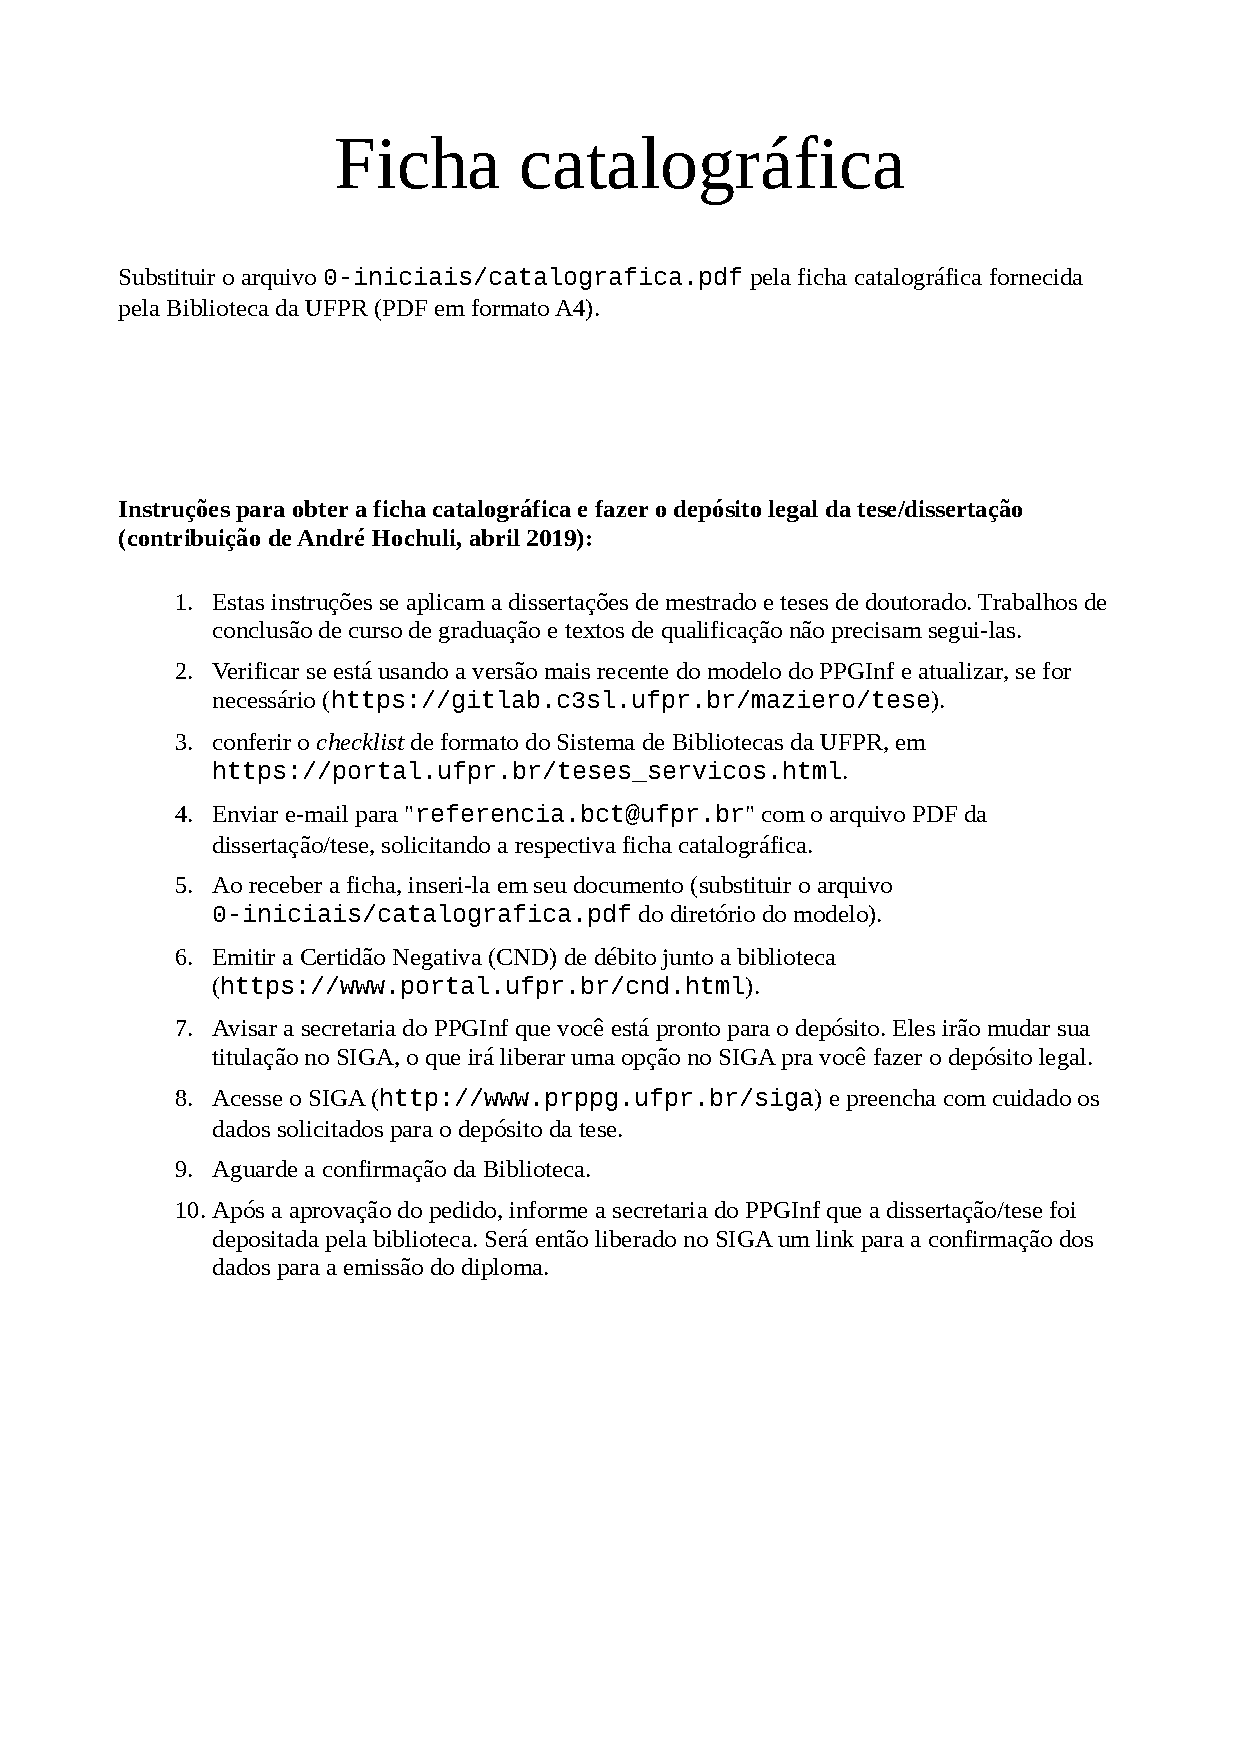
\includepdf[noautoscale]{0-iniciais/catalografica.pdf}

\end{ficha}

%=====================================================
	% ficha catalográfica
% A ficha de aprovação será fornecida pela secretaria do programa,
% após a defesa e cumprimento dos demais trâmites legais.

\begin{aprovacao}	% só gera conteúdo se for na versão final

% inclusão do termo de aprovação final (arquivo PDF)
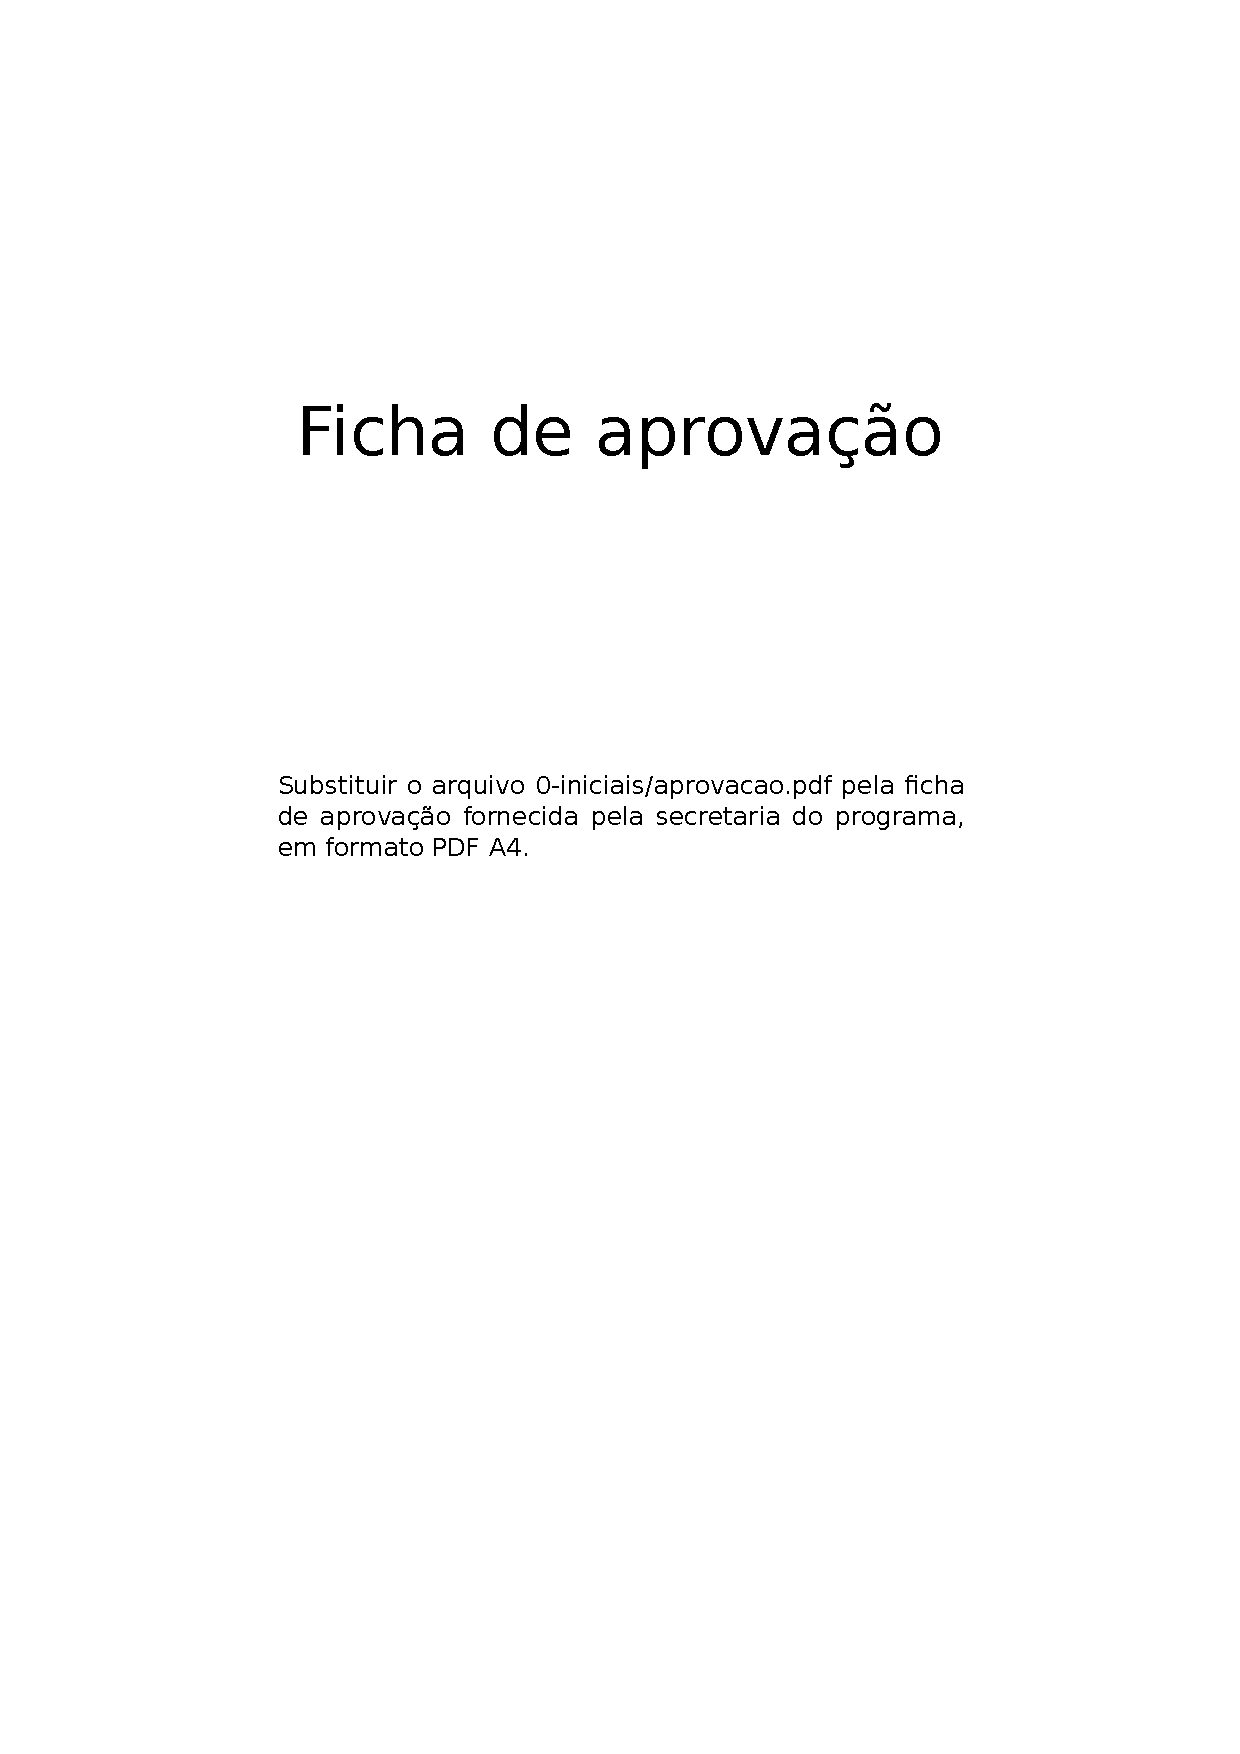
\includepdf[noautoscale]{0-iniciais/aprovacao.pdf}

\end{aprovacao}

%=====================================================
		% folha de aprovação
\begin{dedica}  % só gera conteúdo se for na versão final

A alguém...

\end{dedica}

		% dedicatória
\begin{agradece}	% só gera conteúdo se for na versão final

Inserir os agradecimentos. Os agradecimentos devem ocupar no máximo uma página, devem ser justificados na largura da página e com um afastamento de parágrafo na primeira linha de 1,27 cm. O espaçamento entre linhas deve ser de 1,5 linhas. Não deve haver espaçamento adicional entre parágrafos.

\lipsum[2-5]	% gera um texto aleatório

\end{agradece}

		% agradecimentos

% resumo (português) e abstract (inglês)
\begin{resumo}
	O objetivo deste trabalho é, por meio de três tipos de gráficos de entrada, enfatizar a importância de se analisar a centralidade dos caminhos mínimos. Para isto, foi proposto o uso do algoritmo de Dijkstra para a busca de caminhos mínimos entre todos os pares de vértices em um grafo e para armazenamento e manipulação de dados, foi proposto o uso de dicionários como estrutura de dados mais comum para armazenar os caminhos mínimos com seus respectivos valores de centralidade. O que motiva este trabalho é o fato de que os grafos representam muito bem situações da vida real, como mapas, redes sociais, entre outras. A busca por rotas otimizadas em mapas é um exemplo do escopo de grafos que cobre o problema de caminhos mínimos. É muito interessante analisar os valores de centralidades dos caminhos mínimos em um grafo e, um exemplo disto, no tráfego de dados em uma rede cabeada, existem pontos (rotas) nesta infraestrutura que devem ter estruturas físicas mais robustas para suportar a alta transferência de dados e afins. Pesquisar a centralidade dos caminhos mínimos é uma excelente forma de analisar estes estudos de casos. Os resultados apresentados neste trabalho permitirão visualizar a teoria algorítmica proposta, juntamente com o comportamento da distribuição dos valores de centralidade. \newline \newline
\end{resumo}

\begin{abstract}

The abstract should be the English translation of the ``resumo'', no more, no less.

\lipsum[10-13]	% texto aleatório

\end{abstract}


% listas  de figuras, tabelas, abreviações/siglas, símbolos
\listoffigures				% figuras
\clearpage
\listoftables				% tabelas
%=====================================================

% lista de acrônimos (siglas e abreviações)

\begin{listaacron}

\begin{longtable}[l]{p{0.2\linewidth}p{0.7\linewidth}}
DINF & Departamento de Informática\\
PPGINF & Programa de Pós-Graduação em Informática\\
UFPR & Universidade Federal do Paraná\\
\end{longtable}

\end{listaacron}

%=====================================================
		% acrônimos, deve ser preenchida à mão
%=====================================================

% lista de símbolos

\begin{listasimb}

\begin{longtable}[l]{p{0.2\linewidth}p{0.7\linewidth}}
	$V$					& Conjunto de vértices de um grafo \\
	$E$					& Conjunto de arestas de um grafo \\
	$G(V, E)$			& Um grafo com $V$ vértices e $E$ arestas \\
	$d(v)$ 				& Grau do vértice $v$ \\
	$\pi$ 				& pi \\
	$T_u$ 				& Árvore de caminhos mínimos de um vértice $u$ \\
	$\mathcal{B}_u(v)$	& Dado $T_u$, $\mathcal{B}_u(v)$ é um ramo do vértice $u$ ao vértice $v$ \\
\end{longtable}

\end{listasimb}

%=====================================================
		% símbolos, idem
\tableofcontents			% sumário

%=====================================================

% define estilo do corpo do documento (capítulos e apêndices)
\mainmatter
\pagestyle{mainmatter}

% inclusao de cada capítulo, alterar a gosto (do professor de Metodologia)
\graphicspath{{\currfiledir/images/}}

%----------------------------------------------------------------------------------------
%	Metodologia
%----------------------------------------------------------------------------------------
\chapter{Metodologia}
De um ponto de vista algorítmico e de estruturas de dados, os grafos são amplamente utilizados para representar redes em geral, sejam estas representações de mapas, redes sociais ou até mesmo o fluxo de influências numa rede bibliográfica. O estudo sobre a análise da centralidade de caminhos mínimos é bastante relevante em diversos cenários da vida real. Dado um mapa, por exemplo, existem rotas que são mais comumente usadas por transportes de carga rodoviário, desta forma, espera-se que este trajeto demande de mais frequente manutenção.

Neste trabalho foram implementados e executados, experimentos de conceitos introduzidos em \cite{alane2021}. O problema da centralidade de caminhos mínimos é explorado neste trabalho de um ponto de vista de aplicabilidade, pois o algoritmo e todo seu processo, já em teoria, são extremamente custosos em tempo de execução para grafos muito esparsos. Tal pesquisa busca métodos de análise da centralidade de caminhos mínimos de forma mais eficiente.

Dito isto, este trabalho irá mostrar a aplicação de um algoritmo exato em três exemplos de grafos. O objetivo central é investigar, mesmo que preliminarmente, a distribuição dos valores de centralidade de caminhos mínimos. Os grafos que serão utilizados neste trabalho não são direcionados.

Para apresentação visual e conceitual da metodologia serão utilizados: um grafo simples, com 5 vértices; o modelo de grafo do clube de karatê de Zachary, que é uma rede social de um clube universitário de karatê \cite{zachary2009} e a rede de jogos de futebol americano entre as faculdades da Divisão IA durante a temporada regular do outono de 2000 \cite{networkxfootball2021}.

%----------------------------------------------------------------------------------------
%	Algoritmo
%----------------------------------------------------------------------------------------
\section{Algoritmo}
Dados os grafos de entrada, a ideia geral do trabalho é obter todos os possíveis caminhos mínimos, isto é, executar o algoritmo de Dijkstra para cada um dos $n$ vértices do grafo. Como já mencionado, o algoritmo de Dijkstra, dado um vértice alvo, constrói uma árvore de caminhos mínimos, sendo cada percurso da raiz até os nós da árvore um caminho mínimo da raiz ao nó. Em situações em que o grafo é conexo, a quantidade de caminhos mínimos de um vértice para todos os demais é de $n - 1$. Este processo será executado $n$ vezes, isto é, para todos os vértices do grafo.


A função \emph{main()} serve como chamada central de outras subfunções que fazem o tratamento dos dados e que serão explicadas em sequência. De forma geral, esta função faz a construção de um grafo (linhas 2 - 4), determina os caminhos mínimos para todos os vértices (linhas 5 - 8), faz a computação de centralidade dos caminhos mínimos de um grafo (linha 7) e exibe, na saída padrão, todos os caminhos mínimos com seus respectivos valores de centralidade (linha 8).

\begin{lstlisting}[caption={Função central para chamada de subfunções.}]
	def main() -> None:
		G = simple_graph_generator()
		G = karate_club_graph_generator()
		G = football_graph_generator()

		dijkstraTrees = get_dijkstra_trees_from_a_graph(G)
		shortestPaths = get_shortest_paths(dijkstraTrees)
		all_shortest_paths_centrality(shortestPaths)
		print_all_paths_and_centrality(shortestPaths)
\end{lstlisting}

Para a geração de grafos de entrada, o código proposto neste trabalho possui 3 funções: o Algoritmo~\ref{sec4:funcao_simple_graph_generator}~\emph{($simple\textunderscore graph\textunderscore generator()$)}, o Algoritmo~\ref{sec4:funcao_karate_club_graph_generator}~\emph{($karate\textunderscore club\textunderscore graph\textunderscore generator()$)} e o Algoritmo~\ref{sec4:funcao_rede_futebol}~\emph{($football\textunderscore graph\textunderscore generator()$)}. Estas funções usam a biblioteca \emph{NetworkX} para construção manual do grafo simples, do clube de karatê, predefinidos na biblioteca, e chamada por fonte externa do grafo da rede de jogos de futebol americano.

\begin{lstlisting}[caption={Função para gerar um grafo simples.}\label{sec4:funcao_simple_graph_generator}]
	def simple_graph_generator():
		G = nx.Graph()
		G.add_edge(1, 2)
		G.add_edge(1, 3)
		G.add_edge(1, 5)
		G.add_edge(2, 3)
		G.add_edge(3, 4)
		G.add_edge(4, 5)
		return(G)
\end{lstlisting}

\begin{lstlisting}[caption={Função para gerar o modelo de grafo do clube de karatê de Zachary.}\label{sec4:funcao_karate_club_graph_generator}]
	def karate_club_graph_generator():
		G = nx.karate_club_graph()
		for v in G:
			print(f``{v:4} {G.degree(v):6}'')
		return(G)
\end{lstlisting}

\begin{lstlisting}[caption={Função para gerar o modelo de grafo da rede de futebol americano. Disponível em \cite{networkx2021}}.\label{sec4:funcao_rede_futebol}]
	def football_graph_generator():
		url = ``http://www-personal.umich.edu/~mejn/netdata/football.zip''
		sock = urllib.request.urlopen(url)  # open URL
		s = io.BytesIO(sock.read())  # read into BytesIO ``file''
		sock.close()
		zf = zipfile.ZipFile(s)  # zipfile object
		txt = zf.read(``football.txt'').decode()  # read info file
		gml = zf.read(``football.gml'').decode()  # read gml data
		# throw away bogus first line with # from mejn files
		gml = gml.split(``\n'')[1:]
		G = nx.parse_gml(gml)  # parse gml data
		return G
\end{lstlisting}

Com os grafos de entrada criados, iniciaremos o processo de tratamento destes dados.

Dado um grafo de entrada, o Algoritmo~\ref{sec4:funcao_get_dijkstra_trees_from_a_graph}~(\emph{$get\textunderscore dijkstra\textunderscore trees\textunderscore from\textunderscore a\textunderscore graph()$}) trata os dados de entrada para passar por cada um dos vértices, gerando a árvore de Dijkstra. Estes dados são armazenados em um dicionário, estrutura de dados para armazenamento de dados com indexação por chaves,de caminhos mínimos, indexado pelos rótulos dos vértices.

\begin{lstlisting}[caption={Função para tratar os dados de um grafo de entrada e gerar um dicionário de árvores de Dijkstra, indexado pelos rótulos dos vértices do grafo.}\label{sec4:funcao_get_dijkstra_trees_from_a_graph}]
	def get_dijkstra_trees_from_a_graph(g: dict) -> dict:
		graphDict = {}
		for node in g:
			if node not in graphDict:
				graphDict[node] = single_source_dijkstra(g, node)[1]
		return graphDict
\end{lstlisting}

No próximo passo, o Algoritmo~\ref{sec4:get_shortest_paths_from_dijkstra_trees}~(\emph{$get\textunderscore shortest\textunderscore paths\textunderscore from\textunderscore dijkstra\textunderscore trees()$}) é uma etapa de refinamento dos dados previamente obtidos. Isto é, a partir dos dados do dicionário de caminhos mínimos retornados pela função \emph{$get\textunderscore dijkstra\textunderscore trees\textunderscore from\textunderscore a\textunderscore graph()$}, o algoritmo faz operações de normalização textual, como retirada de colchetes nos nomes dos caminhos mínimos, por exemplo.

\begin{lstlisting}[caption={Função para refinamento do dicionário de caminhos mínimos.}\label{sec4:get_shortest_paths_from_dijkstra_trees}]
	class PathInfo:
		def __init__(self, centrality: int, numNodes: int) -> None:
			self.centrality = centrality
			self.numNodes = numNodes

	def get_shortest_paths_from_dijkstra_trees(graphDict: dict) -> dict:
		pathDict = {}

		for i in graphDict.values():
			for j in i.values():
				path = str(j).replace(``['', ``'').replace(``]'', ``'')
				if path not in pathDict and len(path) > 1:
					newPathInfo = PathInfo(0, len(j))
					pathDict[path] = newPathInfo

		return pathDict
\end{lstlisting}

Tendo-se os dados refinados, a última etapa visa calcular a centralidades dos caminhos mínimos, no Algoritmo~\ref{sec4:all_shortest_paths_centrality} (\emph{$all\textunderscore shortest\textunderscore paths\textunderscore centrality()$}). A centralidades dos caminhos mínimos do grafo é calculada da seguinte forma: para cada caminho mínimo $cm_1$, verifique em todos os demais caminhos mínimos se $cm_1$ está presente como subcaminho mínimo (\emph{linhas 2 - 5}); em caso positivo, contabilize $+1$ na centralidade de $cm_1$ (\emph{linha 6}). Estas etapas são repetidas para todos os demais caminhos mínimos (\emph{linhas 2 - 6}). Feito isto, os valores são normalizados (\emph{linhas 11 - 13}), para que os valores de ponderação estejam entre $0$ e $1$. Ou seja, quanto mais próximo de $1$, maior a centralidade do caminho mínimo.

\begin{lstlisting}[caption={Função para cálculo da centralidade dos caminhos mínimos.}\label{sec4:all_shortest_paths_centrality}]
def all_shortest_paths_centrality(pathDict: dict) -> dict:
	# Check if i is contained in j. If so, add one
	for i in pathDict:
		for j in pathDict:
			if i in j:
				pathDict[i].centrality += 1

	# Get the number of Dijkstra trees
	numTrees = len(pathDict)

	# Normalizing centrality values
	for path in pathDict:
		pathDict[path].centrality /= numTrees * pathDict[path].numNodes
\end{lstlisting}			            % Introdução
\graphicspath{{\currfiledir/images/}}

%----------------------------------------------------------------------------------------
%	Metodologia
%----------------------------------------------------------------------------------------
\chapter{Metodologia}
De um ponto de vista algorítmico e de estruturas de dados, os grafos são amplamente utilizados para representar redes em geral, sejam estas representações de mapas, redes sociais ou até mesmo o fluxo de influências numa rede bibliográfica. O estudo sobre a análise da centralidade de caminhos mínimos é bastante relevante em diversos cenários da vida real. Dado um mapa, por exemplo, existem rotas que são mais comumente usadas por transportes de carga rodoviário, desta forma, espera-se que este trajeto demande de mais frequente manutenção.

Neste trabalho foram implementados e executados, experimentos de conceitos introduzidos em \cite{alane2021}. O problema da centralidade de caminhos mínimos é explorado neste trabalho de um ponto de vista de aplicabilidade, pois o algoritmo e todo seu processo, já em teoria, são extremamente custosos em tempo de execução para grafos muito esparsos. Tal pesquisa busca métodos de análise da centralidade de caminhos mínimos de forma mais eficiente.

Dito isto, este trabalho irá mostrar a aplicação de um algoritmo exato em três exemplos de grafos. O objetivo central é investigar, mesmo que preliminarmente, a distribuição dos valores de centralidade de caminhos mínimos. Os grafos que serão utilizados neste trabalho não são direcionados.

Para apresentação visual e conceitual da metodologia serão utilizados: um grafo simples, com 5 vértices; o modelo de grafo do clube de karatê de Zachary, que é uma rede social de um clube universitário de karatê \cite{zachary2009} e a rede de jogos de futebol americano entre as faculdades da Divisão IA durante a temporada regular do outono de 2000 \cite{networkxfootball2021}.

%----------------------------------------------------------------------------------------
%	Algoritmo
%----------------------------------------------------------------------------------------
\section{Algoritmo}
Dados os grafos de entrada, a ideia geral do trabalho é obter todos os possíveis caminhos mínimos, isto é, executar o algoritmo de Dijkstra para cada um dos $n$ vértices do grafo. Como já mencionado, o algoritmo de Dijkstra, dado um vértice alvo, constrói uma árvore de caminhos mínimos, sendo cada percurso da raiz até os nós da árvore um caminho mínimo da raiz ao nó. Em situações em que o grafo é conexo, a quantidade de caminhos mínimos de um vértice para todos os demais é de $n - 1$. Este processo será executado $n$ vezes, isto é, para todos os vértices do grafo.


A função \emph{main()} serve como chamada central de outras subfunções que fazem o tratamento dos dados e que serão explicadas em sequência. De forma geral, esta função faz a construção de um grafo (linhas 2 - 4), determina os caminhos mínimos para todos os vértices (linhas 5 - 8), faz a computação de centralidade dos caminhos mínimos de um grafo (linha 7) e exibe, na saída padrão, todos os caminhos mínimos com seus respectivos valores de centralidade (linha 8).

\begin{lstlisting}[caption={Função central para chamada de subfunções.}]
	def main() -> None:
		G = simple_graph_generator()
		G = karate_club_graph_generator()
		G = football_graph_generator()

		dijkstraTrees = get_dijkstra_trees_from_a_graph(G)
		shortestPaths = get_shortest_paths(dijkstraTrees)
		all_shortest_paths_centrality(shortestPaths)
		print_all_paths_and_centrality(shortestPaths)
\end{lstlisting}

Para a geração de grafos de entrada, o código proposto neste trabalho possui 3 funções: o Algoritmo~\ref{sec4:funcao_simple_graph_generator}~\emph{($simple\textunderscore graph\textunderscore generator()$)}, o Algoritmo~\ref{sec4:funcao_karate_club_graph_generator}~\emph{($karate\textunderscore club\textunderscore graph\textunderscore generator()$)} e o Algoritmo~\ref{sec4:funcao_rede_futebol}~\emph{($football\textunderscore graph\textunderscore generator()$)}. Estas funções usam a biblioteca \emph{NetworkX} para construção manual do grafo simples, do clube de karatê, predefinidos na biblioteca, e chamada por fonte externa do grafo da rede de jogos de futebol americano.

\begin{lstlisting}[caption={Função para gerar um grafo simples.}\label{sec4:funcao_simple_graph_generator}]
	def simple_graph_generator():
		G = nx.Graph()
		G.add_edge(1, 2)
		G.add_edge(1, 3)
		G.add_edge(1, 5)
		G.add_edge(2, 3)
		G.add_edge(3, 4)
		G.add_edge(4, 5)
		return(G)
\end{lstlisting}

\begin{lstlisting}[caption={Função para gerar o modelo de grafo do clube de karatê de Zachary.}\label{sec4:funcao_karate_club_graph_generator}]
	def karate_club_graph_generator():
		G = nx.karate_club_graph()
		for v in G:
			print(f``{v:4} {G.degree(v):6}'')
		return(G)
\end{lstlisting}

\begin{lstlisting}[caption={Função para gerar o modelo de grafo da rede de futebol americano. Disponível em \cite{networkx2021}}.\label{sec4:funcao_rede_futebol}]
	def football_graph_generator():
		url = ``http://www-personal.umich.edu/~mejn/netdata/football.zip''
		sock = urllib.request.urlopen(url)  # open URL
		s = io.BytesIO(sock.read())  # read into BytesIO ``file''
		sock.close()
		zf = zipfile.ZipFile(s)  # zipfile object
		txt = zf.read(``football.txt'').decode()  # read info file
		gml = zf.read(``football.gml'').decode()  # read gml data
		# throw away bogus first line with # from mejn files
		gml = gml.split(``\n'')[1:]
		G = nx.parse_gml(gml)  # parse gml data
		return G
\end{lstlisting}

Com os grafos de entrada criados, iniciaremos o processo de tratamento destes dados.

Dado um grafo de entrada, o Algoritmo~\ref{sec4:funcao_get_dijkstra_trees_from_a_graph}~(\emph{$get\textunderscore dijkstra\textunderscore trees\textunderscore from\textunderscore a\textunderscore graph()$}) trata os dados de entrada para passar por cada um dos vértices, gerando a árvore de Dijkstra. Estes dados são armazenados em um dicionário, estrutura de dados para armazenamento de dados com indexação por chaves,de caminhos mínimos, indexado pelos rótulos dos vértices.

\begin{lstlisting}[caption={Função para tratar os dados de um grafo de entrada e gerar um dicionário de árvores de Dijkstra, indexado pelos rótulos dos vértices do grafo.}\label{sec4:funcao_get_dijkstra_trees_from_a_graph}]
	def get_dijkstra_trees_from_a_graph(g: dict) -> dict:
		graphDict = {}
		for node in g:
			if node not in graphDict:
				graphDict[node] = single_source_dijkstra(g, node)[1]
		return graphDict
\end{lstlisting}

No próximo passo, o Algoritmo~\ref{sec4:get_shortest_paths_from_dijkstra_trees}~(\emph{$get\textunderscore shortest\textunderscore paths\textunderscore from\textunderscore dijkstra\textunderscore trees()$}) é uma etapa de refinamento dos dados previamente obtidos. Isto é, a partir dos dados do dicionário de caminhos mínimos retornados pela função \emph{$get\textunderscore dijkstra\textunderscore trees\textunderscore from\textunderscore a\textunderscore graph()$}, o algoritmo faz operações de normalização textual, como retirada de colchetes nos nomes dos caminhos mínimos, por exemplo.

\begin{lstlisting}[caption={Função para refinamento do dicionário de caminhos mínimos.}\label{sec4:get_shortest_paths_from_dijkstra_trees}]
	class PathInfo:
		def __init__(self, centrality: int, numNodes: int) -> None:
			self.centrality = centrality
			self.numNodes = numNodes

	def get_shortest_paths_from_dijkstra_trees(graphDict: dict) -> dict:
		pathDict = {}

		for i in graphDict.values():
			for j in i.values():
				path = str(j).replace(``['', ``'').replace(``]'', ``'')
				if path not in pathDict and len(path) > 1:
					newPathInfo = PathInfo(0, len(j))
					pathDict[path] = newPathInfo

		return pathDict
\end{lstlisting}

Tendo-se os dados refinados, a última etapa visa calcular a centralidades dos caminhos mínimos, no Algoritmo~\ref{sec4:all_shortest_paths_centrality} (\emph{$all\textunderscore shortest\textunderscore paths\textunderscore centrality()$}). A centralidades dos caminhos mínimos do grafo é calculada da seguinte forma: para cada caminho mínimo $cm_1$, verifique em todos os demais caminhos mínimos se $cm_1$ está presente como subcaminho mínimo (\emph{linhas 2 - 5}); em caso positivo, contabilize $+1$ na centralidade de $cm_1$ (\emph{linha 6}). Estas etapas são repetidas para todos os demais caminhos mínimos (\emph{linhas 2 - 6}). Feito isto, os valores são normalizados (\emph{linhas 11 - 13}), para que os valores de ponderação estejam entre $0$ e $1$. Ou seja, quanto mais próximo de $1$, maior a centralidade do caminho mínimo.

\begin{lstlisting}[caption={Função para cálculo da centralidade dos caminhos mínimos.}\label{sec4:all_shortest_paths_centrality}]
def all_shortest_paths_centrality(pathDict: dict) -> dict:
	# Check if i is contained in j. If so, add one
	for i in pathDict:
		for j in pathDict:
			if i in j:
				pathDict[i].centrality += 1

	# Get the number of Dijkstra trees
	numTrees = len(pathDict)

	# Normalizing centrality values
	for path in pathDict:
		pathDict[path].centrality /= numTrees * pathDict[path].numNodes
\end{lstlisting}      % Conceitos Introdutórios
\graphicspath{{\currfiledir/images/}}

%----------------------------------------------------------------------------------------
%	Metodologia
%----------------------------------------------------------------------------------------
\chapter{Metodologia}
De um ponto de vista algorítmico e de estruturas de dados, os grafos são amplamente utilizados para representar redes em geral, sejam estas representações de mapas, redes sociais ou até mesmo o fluxo de influências numa rede bibliográfica. O estudo sobre a análise da centralidade de caminhos mínimos é bastante relevante em diversos cenários da vida real. Dado um mapa, por exemplo, existem rotas que são mais comumente usadas por transportes de carga rodoviário, desta forma, espera-se que este trajeto demande de mais frequente manutenção.

Neste trabalho foram implementados e executados, experimentos de conceitos introduzidos em \cite{alane2021}. O problema da centralidade de caminhos mínimos é explorado neste trabalho de um ponto de vista de aplicabilidade, pois o algoritmo e todo seu processo, já em teoria, são extremamente custosos em tempo de execução para grafos muito esparsos. Tal pesquisa busca métodos de análise da centralidade de caminhos mínimos de forma mais eficiente.

Dito isto, este trabalho irá mostrar a aplicação de um algoritmo exato em três exemplos de grafos. O objetivo central é investigar, mesmo que preliminarmente, a distribuição dos valores de centralidade de caminhos mínimos. Os grafos que serão utilizados neste trabalho não são direcionados.

Para apresentação visual e conceitual da metodologia serão utilizados: um grafo simples, com 5 vértices; o modelo de grafo do clube de karatê de Zachary, que é uma rede social de um clube universitário de karatê \cite{zachary2009} e a rede de jogos de futebol americano entre as faculdades da Divisão IA durante a temporada regular do outono de 2000 \cite{networkxfootball2021}.

%----------------------------------------------------------------------------------------
%	Algoritmo
%----------------------------------------------------------------------------------------
\section{Algoritmo}
Dados os grafos de entrada, a ideia geral do trabalho é obter todos os possíveis caminhos mínimos, isto é, executar o algoritmo de Dijkstra para cada um dos $n$ vértices do grafo. Como já mencionado, o algoritmo de Dijkstra, dado um vértice alvo, constrói uma árvore de caminhos mínimos, sendo cada percurso da raiz até os nós da árvore um caminho mínimo da raiz ao nó. Em situações em que o grafo é conexo, a quantidade de caminhos mínimos de um vértice para todos os demais é de $n - 1$. Este processo será executado $n$ vezes, isto é, para todos os vértices do grafo.


A função \emph{main()} serve como chamada central de outras subfunções que fazem o tratamento dos dados e que serão explicadas em sequência. De forma geral, esta função faz a construção de um grafo (linhas 2 - 4), determina os caminhos mínimos para todos os vértices (linhas 5 - 8), faz a computação de centralidade dos caminhos mínimos de um grafo (linha 7) e exibe, na saída padrão, todos os caminhos mínimos com seus respectivos valores de centralidade (linha 8).

\begin{lstlisting}[caption={Função central para chamada de subfunções.}]
	def main() -> None:
		G = simple_graph_generator()
		G = karate_club_graph_generator()
		G = football_graph_generator()

		dijkstraTrees = get_dijkstra_trees_from_a_graph(G)
		shortestPaths = get_shortest_paths(dijkstraTrees)
		all_shortest_paths_centrality(shortestPaths)
		print_all_paths_and_centrality(shortestPaths)
\end{lstlisting}

Para a geração de grafos de entrada, o código proposto neste trabalho possui 3 funções: o Algoritmo~\ref{sec4:funcao_simple_graph_generator}~\emph{($simple\textunderscore graph\textunderscore generator()$)}, o Algoritmo~\ref{sec4:funcao_karate_club_graph_generator}~\emph{($karate\textunderscore club\textunderscore graph\textunderscore generator()$)} e o Algoritmo~\ref{sec4:funcao_rede_futebol}~\emph{($football\textunderscore graph\textunderscore generator()$)}. Estas funções usam a biblioteca \emph{NetworkX} para construção manual do grafo simples, do clube de karatê, predefinidos na biblioteca, e chamada por fonte externa do grafo da rede de jogos de futebol americano.

\begin{lstlisting}[caption={Função para gerar um grafo simples.}\label{sec4:funcao_simple_graph_generator}]
	def simple_graph_generator():
		G = nx.Graph()
		G.add_edge(1, 2)
		G.add_edge(1, 3)
		G.add_edge(1, 5)
		G.add_edge(2, 3)
		G.add_edge(3, 4)
		G.add_edge(4, 5)
		return(G)
\end{lstlisting}

\begin{lstlisting}[caption={Função para gerar o modelo de grafo do clube de karatê de Zachary.}\label{sec4:funcao_karate_club_graph_generator}]
	def karate_club_graph_generator():
		G = nx.karate_club_graph()
		for v in G:
			print(f``{v:4} {G.degree(v):6}'')
		return(G)
\end{lstlisting}

\begin{lstlisting}[caption={Função para gerar o modelo de grafo da rede de futebol americano. Disponível em \cite{networkx2021}}.\label{sec4:funcao_rede_futebol}]
	def football_graph_generator():
		url = ``http://www-personal.umich.edu/~mejn/netdata/football.zip''
		sock = urllib.request.urlopen(url)  # open URL
		s = io.BytesIO(sock.read())  # read into BytesIO ``file''
		sock.close()
		zf = zipfile.ZipFile(s)  # zipfile object
		txt = zf.read(``football.txt'').decode()  # read info file
		gml = zf.read(``football.gml'').decode()  # read gml data
		# throw away bogus first line with # from mejn files
		gml = gml.split(``\n'')[1:]
		G = nx.parse_gml(gml)  # parse gml data
		return G
\end{lstlisting}

Com os grafos de entrada criados, iniciaremos o processo de tratamento destes dados.

Dado um grafo de entrada, o Algoritmo~\ref{sec4:funcao_get_dijkstra_trees_from_a_graph}~(\emph{$get\textunderscore dijkstra\textunderscore trees\textunderscore from\textunderscore a\textunderscore graph()$}) trata os dados de entrada para passar por cada um dos vértices, gerando a árvore de Dijkstra. Estes dados são armazenados em um dicionário, estrutura de dados para armazenamento de dados com indexação por chaves,de caminhos mínimos, indexado pelos rótulos dos vértices.

\begin{lstlisting}[caption={Função para tratar os dados de um grafo de entrada e gerar um dicionário de árvores de Dijkstra, indexado pelos rótulos dos vértices do grafo.}\label{sec4:funcao_get_dijkstra_trees_from_a_graph}]
	def get_dijkstra_trees_from_a_graph(g: dict) -> dict:
		graphDict = {}
		for node in g:
			if node not in graphDict:
				graphDict[node] = single_source_dijkstra(g, node)[1]
		return graphDict
\end{lstlisting}

No próximo passo, o Algoritmo~\ref{sec4:get_shortest_paths_from_dijkstra_trees}~(\emph{$get\textunderscore shortest\textunderscore paths\textunderscore from\textunderscore dijkstra\textunderscore trees()$}) é uma etapa de refinamento dos dados previamente obtidos. Isto é, a partir dos dados do dicionário de caminhos mínimos retornados pela função \emph{$get\textunderscore dijkstra\textunderscore trees\textunderscore from\textunderscore a\textunderscore graph()$}, o algoritmo faz operações de normalização textual, como retirada de colchetes nos nomes dos caminhos mínimos, por exemplo.

\begin{lstlisting}[caption={Função para refinamento do dicionário de caminhos mínimos.}\label{sec4:get_shortest_paths_from_dijkstra_trees}]
	class PathInfo:
		def __init__(self, centrality: int, numNodes: int) -> None:
			self.centrality = centrality
			self.numNodes = numNodes

	def get_shortest_paths_from_dijkstra_trees(graphDict: dict) -> dict:
		pathDict = {}

		for i in graphDict.values():
			for j in i.values():
				path = str(j).replace(``['', ``'').replace(``]'', ``'')
				if path not in pathDict and len(path) > 1:
					newPathInfo = PathInfo(0, len(j))
					pathDict[path] = newPathInfo

		return pathDict
\end{lstlisting}

Tendo-se os dados refinados, a última etapa visa calcular a centralidades dos caminhos mínimos, no Algoritmo~\ref{sec4:all_shortest_paths_centrality} (\emph{$all\textunderscore shortest\textunderscore paths\textunderscore centrality()$}). A centralidades dos caminhos mínimos do grafo é calculada da seguinte forma: para cada caminho mínimo $cm_1$, verifique em todos os demais caminhos mínimos se $cm_1$ está presente como subcaminho mínimo (\emph{linhas 2 - 5}); em caso positivo, contabilize $+1$ na centralidade de $cm_1$ (\emph{linha 6}). Estas etapas são repetidas para todos os demais caminhos mínimos (\emph{linhas 2 - 6}). Feito isto, os valores são normalizados (\emph{linhas 11 - 13}), para que os valores de ponderação estejam entre $0$ e $1$. Ou seja, quanto mais próximo de $1$, maior a centralidade do caminho mínimo.

\begin{lstlisting}[caption={Função para cálculo da centralidade dos caminhos mínimos.}\label{sec4:all_shortest_paths_centrality}]
def all_shortest_paths_centrality(pathDict: dict) -> dict:
	# Check if i is contained in j. If so, add one
	for i in pathDict:
		for j in pathDict:
			if i in j:
				pathDict[i].centrality += 1

	# Get the number of Dijkstra trees
	numTrees = len(pathDict)

	# Normalizing centrality values
	for path in pathDict:
		pathDict[path].centrality /= numTrees * pathDict[path].numNodes
\end{lstlisting}			        % Caminhos Mínimos
\graphicspath{{\currfiledir/images/}}

%----------------------------------------------------------------------------------------
%	Metodologia
%----------------------------------------------------------------------------------------
\chapter{Metodologia}
De um ponto de vista algorítmico e de estruturas de dados, os grafos são amplamente utilizados para representar redes em geral, sejam estas representações de mapas, redes sociais ou até mesmo o fluxo de influências numa rede bibliográfica. O estudo sobre a análise da centralidade de caminhos mínimos é bastante relevante em diversos cenários da vida real. Dado um mapa, por exemplo, existem rotas que são mais comumente usadas por transportes de carga rodoviário, desta forma, espera-se que este trajeto demande de mais frequente manutenção.

Neste trabalho foram implementados e executados, experimentos de conceitos introduzidos em \cite{alane2021}. O problema da centralidade de caminhos mínimos é explorado neste trabalho de um ponto de vista de aplicabilidade, pois o algoritmo e todo seu processo, já em teoria, são extremamente custosos em tempo de execução para grafos muito esparsos. Tal pesquisa busca métodos de análise da centralidade de caminhos mínimos de forma mais eficiente.

Dito isto, este trabalho irá mostrar a aplicação de um algoritmo exato em três exemplos de grafos. O objetivo central é investigar, mesmo que preliminarmente, a distribuição dos valores de centralidade de caminhos mínimos. Os grafos que serão utilizados neste trabalho não são direcionados.

Para apresentação visual e conceitual da metodologia serão utilizados: um grafo simples, com 5 vértices; o modelo de grafo do clube de karatê de Zachary, que é uma rede social de um clube universitário de karatê \cite{zachary2009} e a rede de jogos de futebol americano entre as faculdades da Divisão IA durante a temporada regular do outono de 2000 \cite{networkxfootball2021}.

%----------------------------------------------------------------------------------------
%	Algoritmo
%----------------------------------------------------------------------------------------
\section{Algoritmo}
Dados os grafos de entrada, a ideia geral do trabalho é obter todos os possíveis caminhos mínimos, isto é, executar o algoritmo de Dijkstra para cada um dos $n$ vértices do grafo. Como já mencionado, o algoritmo de Dijkstra, dado um vértice alvo, constrói uma árvore de caminhos mínimos, sendo cada percurso da raiz até os nós da árvore um caminho mínimo da raiz ao nó. Em situações em que o grafo é conexo, a quantidade de caminhos mínimos de um vértice para todos os demais é de $n - 1$. Este processo será executado $n$ vezes, isto é, para todos os vértices do grafo.


A função \emph{main()} serve como chamada central de outras subfunções que fazem o tratamento dos dados e que serão explicadas em sequência. De forma geral, esta função faz a construção de um grafo (linhas 2 - 4), determina os caminhos mínimos para todos os vértices (linhas 5 - 8), faz a computação de centralidade dos caminhos mínimos de um grafo (linha 7) e exibe, na saída padrão, todos os caminhos mínimos com seus respectivos valores de centralidade (linha 8).

\begin{lstlisting}[caption={Função central para chamada de subfunções.}]
	def main() -> None:
		G = simple_graph_generator()
		G = karate_club_graph_generator()
		G = football_graph_generator()

		dijkstraTrees = get_dijkstra_trees_from_a_graph(G)
		shortestPaths = get_shortest_paths(dijkstraTrees)
		all_shortest_paths_centrality(shortestPaths)
		print_all_paths_and_centrality(shortestPaths)
\end{lstlisting}

Para a geração de grafos de entrada, o código proposto neste trabalho possui 3 funções: o Algoritmo~\ref{sec4:funcao_simple_graph_generator}~\emph{($simple\textunderscore graph\textunderscore generator()$)}, o Algoritmo~\ref{sec4:funcao_karate_club_graph_generator}~\emph{($karate\textunderscore club\textunderscore graph\textunderscore generator()$)} e o Algoritmo~\ref{sec4:funcao_rede_futebol}~\emph{($football\textunderscore graph\textunderscore generator()$)}. Estas funções usam a biblioteca \emph{NetworkX} para construção manual do grafo simples, do clube de karatê, predefinidos na biblioteca, e chamada por fonte externa do grafo da rede de jogos de futebol americano.

\begin{lstlisting}[caption={Função para gerar um grafo simples.}\label{sec4:funcao_simple_graph_generator}]
	def simple_graph_generator():
		G = nx.Graph()
		G.add_edge(1, 2)
		G.add_edge(1, 3)
		G.add_edge(1, 5)
		G.add_edge(2, 3)
		G.add_edge(3, 4)
		G.add_edge(4, 5)
		return(G)
\end{lstlisting}

\begin{lstlisting}[caption={Função para gerar o modelo de grafo do clube de karatê de Zachary.}\label{sec4:funcao_karate_club_graph_generator}]
	def karate_club_graph_generator():
		G = nx.karate_club_graph()
		for v in G:
			print(f``{v:4} {G.degree(v):6}'')
		return(G)
\end{lstlisting}

\begin{lstlisting}[caption={Função para gerar o modelo de grafo da rede de futebol americano. Disponível em \cite{networkx2021}}.\label{sec4:funcao_rede_futebol}]
	def football_graph_generator():
		url = ``http://www-personal.umich.edu/~mejn/netdata/football.zip''
		sock = urllib.request.urlopen(url)  # open URL
		s = io.BytesIO(sock.read())  # read into BytesIO ``file''
		sock.close()
		zf = zipfile.ZipFile(s)  # zipfile object
		txt = zf.read(``football.txt'').decode()  # read info file
		gml = zf.read(``football.gml'').decode()  # read gml data
		# throw away bogus first line with # from mejn files
		gml = gml.split(``\n'')[1:]
		G = nx.parse_gml(gml)  # parse gml data
		return G
\end{lstlisting}

Com os grafos de entrada criados, iniciaremos o processo de tratamento destes dados.

Dado um grafo de entrada, o Algoritmo~\ref{sec4:funcao_get_dijkstra_trees_from_a_graph}~(\emph{$get\textunderscore dijkstra\textunderscore trees\textunderscore from\textunderscore a\textunderscore graph()$}) trata os dados de entrada para passar por cada um dos vértices, gerando a árvore de Dijkstra. Estes dados são armazenados em um dicionário, estrutura de dados para armazenamento de dados com indexação por chaves,de caminhos mínimos, indexado pelos rótulos dos vértices.

\begin{lstlisting}[caption={Função para tratar os dados de um grafo de entrada e gerar um dicionário de árvores de Dijkstra, indexado pelos rótulos dos vértices do grafo.}\label{sec4:funcao_get_dijkstra_trees_from_a_graph}]
	def get_dijkstra_trees_from_a_graph(g: dict) -> dict:
		graphDict = {}
		for node in g:
			if node not in graphDict:
				graphDict[node] = single_source_dijkstra(g, node)[1]
		return graphDict
\end{lstlisting}

No próximo passo, o Algoritmo~\ref{sec4:get_shortest_paths_from_dijkstra_trees}~(\emph{$get\textunderscore shortest\textunderscore paths\textunderscore from\textunderscore dijkstra\textunderscore trees()$}) é uma etapa de refinamento dos dados previamente obtidos. Isto é, a partir dos dados do dicionário de caminhos mínimos retornados pela função \emph{$get\textunderscore dijkstra\textunderscore trees\textunderscore from\textunderscore a\textunderscore graph()$}, o algoritmo faz operações de normalização textual, como retirada de colchetes nos nomes dos caminhos mínimos, por exemplo.

\begin{lstlisting}[caption={Função para refinamento do dicionário de caminhos mínimos.}\label{sec4:get_shortest_paths_from_dijkstra_trees}]
	class PathInfo:
		def __init__(self, centrality: int, numNodes: int) -> None:
			self.centrality = centrality
			self.numNodes = numNodes

	def get_shortest_paths_from_dijkstra_trees(graphDict: dict) -> dict:
		pathDict = {}

		for i in graphDict.values():
			for j in i.values():
				path = str(j).replace(``['', ``'').replace(``]'', ``'')
				if path not in pathDict and len(path) > 1:
					newPathInfo = PathInfo(0, len(j))
					pathDict[path] = newPathInfo

		return pathDict
\end{lstlisting}

Tendo-se os dados refinados, a última etapa visa calcular a centralidades dos caminhos mínimos, no Algoritmo~\ref{sec4:all_shortest_paths_centrality} (\emph{$all\textunderscore shortest\textunderscore paths\textunderscore centrality()$}). A centralidades dos caminhos mínimos do grafo é calculada da seguinte forma: para cada caminho mínimo $cm_1$, verifique em todos os demais caminhos mínimos se $cm_1$ está presente como subcaminho mínimo (\emph{linhas 2 - 5}); em caso positivo, contabilize $+1$ na centralidade de $cm_1$ (\emph{linha 6}). Estas etapas são repetidas para todos os demais caminhos mínimos (\emph{linhas 2 - 6}). Feito isto, os valores são normalizados (\emph{linhas 11 - 13}), para que os valores de ponderação estejam entre $0$ e $1$. Ou seja, quanto mais próximo de $1$, maior a centralidade do caminho mínimo.

\begin{lstlisting}[caption={Função para cálculo da centralidade dos caminhos mínimos.}\label{sec4:all_shortest_paths_centrality}]
def all_shortest_paths_centrality(pathDict: dict) -> dict:
	# Check if i is contained in j. If so, add one
	for i in pathDict:
		for j in pathDict:
			if i in j:
				pathDict[i].centrality += 1

	# Get the number of Dijkstra trees
	numTrees = len(pathDict)

	# Normalizing centrality values
	for path in pathDict:
		pathDict[path].centrality /= numTrees * pathDict[path].numNodes
\end{lstlisting}			            % Metodologia
\graphicspath{{\currfiledir/images/}}

%----------------------------------------------------------------------------------------
%	Metodologia
%----------------------------------------------------------------------------------------
\chapter{Metodologia}
De um ponto de vista algorítmico e de estruturas de dados, os grafos são amplamente utilizados para representar redes em geral, sejam estas representações de mapas, redes sociais ou até mesmo o fluxo de influências numa rede bibliográfica. O estudo sobre a análise da centralidade de caminhos mínimos é bastante relevante em diversos cenários da vida real. Dado um mapa, por exemplo, existem rotas que são mais comumente usadas por transportes de carga rodoviário, desta forma, espera-se que este trajeto demande de mais frequente manutenção.

Neste trabalho foram implementados e executados, experimentos de conceitos introduzidos em \cite{alane2021}. O problema da centralidade de caminhos mínimos é explorado neste trabalho de um ponto de vista de aplicabilidade, pois o algoritmo e todo seu processo, já em teoria, são extremamente custosos em tempo de execução para grafos muito esparsos. Tal pesquisa busca métodos de análise da centralidade de caminhos mínimos de forma mais eficiente.

Dito isto, este trabalho irá mostrar a aplicação de um algoritmo exato em três exemplos de grafos. O objetivo central é investigar, mesmo que preliminarmente, a distribuição dos valores de centralidade de caminhos mínimos. Os grafos que serão utilizados neste trabalho não são direcionados.

Para apresentação visual e conceitual da metodologia serão utilizados: um grafo simples, com 5 vértices; o modelo de grafo do clube de karatê de Zachary, que é uma rede social de um clube universitário de karatê \cite{zachary2009} e a rede de jogos de futebol americano entre as faculdades da Divisão IA durante a temporada regular do outono de 2000 \cite{networkxfootball2021}.

%----------------------------------------------------------------------------------------
%	Algoritmo
%----------------------------------------------------------------------------------------
\section{Algoritmo}
Dados os grafos de entrada, a ideia geral do trabalho é obter todos os possíveis caminhos mínimos, isto é, executar o algoritmo de Dijkstra para cada um dos $n$ vértices do grafo. Como já mencionado, o algoritmo de Dijkstra, dado um vértice alvo, constrói uma árvore de caminhos mínimos, sendo cada percurso da raiz até os nós da árvore um caminho mínimo da raiz ao nó. Em situações em que o grafo é conexo, a quantidade de caminhos mínimos de um vértice para todos os demais é de $n - 1$. Este processo será executado $n$ vezes, isto é, para todos os vértices do grafo.


A função \emph{main()} serve como chamada central de outras subfunções que fazem o tratamento dos dados e que serão explicadas em sequência. De forma geral, esta função faz a construção de um grafo (linhas 2 - 4), determina os caminhos mínimos para todos os vértices (linhas 5 - 8), faz a computação de centralidade dos caminhos mínimos de um grafo (linha 7) e exibe, na saída padrão, todos os caminhos mínimos com seus respectivos valores de centralidade (linha 8).

\begin{lstlisting}[caption={Função central para chamada de subfunções.}]
	def main() -> None:
		G = simple_graph_generator()
		G = karate_club_graph_generator()
		G = football_graph_generator()

		dijkstraTrees = get_dijkstra_trees_from_a_graph(G)
		shortestPaths = get_shortest_paths(dijkstraTrees)
		all_shortest_paths_centrality(shortestPaths)
		print_all_paths_and_centrality(shortestPaths)
\end{lstlisting}

Para a geração de grafos de entrada, o código proposto neste trabalho possui 3 funções: o Algoritmo~\ref{sec4:funcao_simple_graph_generator}~\emph{($simple\textunderscore graph\textunderscore generator()$)}, o Algoritmo~\ref{sec4:funcao_karate_club_graph_generator}~\emph{($karate\textunderscore club\textunderscore graph\textunderscore generator()$)} e o Algoritmo~\ref{sec4:funcao_rede_futebol}~\emph{($football\textunderscore graph\textunderscore generator()$)}. Estas funções usam a biblioteca \emph{NetworkX} para construção manual do grafo simples, do clube de karatê, predefinidos na biblioteca, e chamada por fonte externa do grafo da rede de jogos de futebol americano.

\begin{lstlisting}[caption={Função para gerar um grafo simples.}\label{sec4:funcao_simple_graph_generator}]
	def simple_graph_generator():
		G = nx.Graph()
		G.add_edge(1, 2)
		G.add_edge(1, 3)
		G.add_edge(1, 5)
		G.add_edge(2, 3)
		G.add_edge(3, 4)
		G.add_edge(4, 5)
		return(G)
\end{lstlisting}

\begin{lstlisting}[caption={Função para gerar o modelo de grafo do clube de karatê de Zachary.}\label{sec4:funcao_karate_club_graph_generator}]
	def karate_club_graph_generator():
		G = nx.karate_club_graph()
		for v in G:
			print(f``{v:4} {G.degree(v):6}'')
		return(G)
\end{lstlisting}

\begin{lstlisting}[caption={Função para gerar o modelo de grafo da rede de futebol americano. Disponível em \cite{networkx2021}}.\label{sec4:funcao_rede_futebol}]
	def football_graph_generator():
		url = ``http://www-personal.umich.edu/~mejn/netdata/football.zip''
		sock = urllib.request.urlopen(url)  # open URL
		s = io.BytesIO(sock.read())  # read into BytesIO ``file''
		sock.close()
		zf = zipfile.ZipFile(s)  # zipfile object
		txt = zf.read(``football.txt'').decode()  # read info file
		gml = zf.read(``football.gml'').decode()  # read gml data
		# throw away bogus first line with # from mejn files
		gml = gml.split(``\n'')[1:]
		G = nx.parse_gml(gml)  # parse gml data
		return G
\end{lstlisting}

Com os grafos de entrada criados, iniciaremos o processo de tratamento destes dados.

Dado um grafo de entrada, o Algoritmo~\ref{sec4:funcao_get_dijkstra_trees_from_a_graph}~(\emph{$get\textunderscore dijkstra\textunderscore trees\textunderscore from\textunderscore a\textunderscore graph()$}) trata os dados de entrada para passar por cada um dos vértices, gerando a árvore de Dijkstra. Estes dados são armazenados em um dicionário, estrutura de dados para armazenamento de dados com indexação por chaves,de caminhos mínimos, indexado pelos rótulos dos vértices.

\begin{lstlisting}[caption={Função para tratar os dados de um grafo de entrada e gerar um dicionário de árvores de Dijkstra, indexado pelos rótulos dos vértices do grafo.}\label{sec4:funcao_get_dijkstra_trees_from_a_graph}]
	def get_dijkstra_trees_from_a_graph(g: dict) -> dict:
		graphDict = {}
		for node in g:
			if node not in graphDict:
				graphDict[node] = single_source_dijkstra(g, node)[1]
		return graphDict
\end{lstlisting}

No próximo passo, o Algoritmo~\ref{sec4:get_shortest_paths_from_dijkstra_trees}~(\emph{$get\textunderscore shortest\textunderscore paths\textunderscore from\textunderscore dijkstra\textunderscore trees()$}) é uma etapa de refinamento dos dados previamente obtidos. Isto é, a partir dos dados do dicionário de caminhos mínimos retornados pela função \emph{$get\textunderscore dijkstra\textunderscore trees\textunderscore from\textunderscore a\textunderscore graph()$}, o algoritmo faz operações de normalização textual, como retirada de colchetes nos nomes dos caminhos mínimos, por exemplo.

\begin{lstlisting}[caption={Função para refinamento do dicionário de caminhos mínimos.}\label{sec4:get_shortest_paths_from_dijkstra_trees}]
	class PathInfo:
		def __init__(self, centrality: int, numNodes: int) -> None:
			self.centrality = centrality
			self.numNodes = numNodes

	def get_shortest_paths_from_dijkstra_trees(graphDict: dict) -> dict:
		pathDict = {}

		for i in graphDict.values():
			for j in i.values():
				path = str(j).replace(``['', ``'').replace(``]'', ``'')
				if path not in pathDict and len(path) > 1:
					newPathInfo = PathInfo(0, len(j))
					pathDict[path] = newPathInfo

		return pathDict
\end{lstlisting}

Tendo-se os dados refinados, a última etapa visa calcular a centralidades dos caminhos mínimos, no Algoritmo~\ref{sec4:all_shortest_paths_centrality} (\emph{$all\textunderscore shortest\textunderscore paths\textunderscore centrality()$}). A centralidades dos caminhos mínimos do grafo é calculada da seguinte forma: para cada caminho mínimo $cm_1$, verifique em todos os demais caminhos mínimos se $cm_1$ está presente como subcaminho mínimo (\emph{linhas 2 - 5}); em caso positivo, contabilize $+1$ na centralidade de $cm_1$ (\emph{linha 6}). Estas etapas são repetidas para todos os demais caminhos mínimos (\emph{linhas 2 - 6}). Feito isto, os valores são normalizados (\emph{linhas 11 - 13}), para que os valores de ponderação estejam entre $0$ e $1$. Ou seja, quanto mais próximo de $1$, maior a centralidade do caminho mínimo.

\begin{lstlisting}[caption={Função para cálculo da centralidade dos caminhos mínimos.}\label{sec4:all_shortest_paths_centrality}]
def all_shortest_paths_centrality(pathDict: dict) -> dict:
	# Check if i is contained in j. If so, add one
	for i in pathDict:
		for j in pathDict:
			if i in j:
				pathDict[i].centrality += 1

	# Get the number of Dijkstra trees
	numTrees = len(pathDict)

	# Normalizing centrality values
	for path in pathDict:
		pathDict[path].centrality /= numTrees * pathDict[path].numNodes
\end{lstlisting}			            % Resultados
\graphicspath{{\currfiledir/images/}}

%----------------------------------------------------------------------------------------
%	Metodologia
%----------------------------------------------------------------------------------------
\chapter{Metodologia}
De um ponto de vista algorítmico e de estruturas de dados, os grafos são amplamente utilizados para representar redes em geral, sejam estas representações de mapas, redes sociais ou até mesmo o fluxo de influências numa rede bibliográfica. O estudo sobre a análise da centralidade de caminhos mínimos é bastante relevante em diversos cenários da vida real. Dado um mapa, por exemplo, existem rotas que são mais comumente usadas por transportes de carga rodoviário, desta forma, espera-se que este trajeto demande de mais frequente manutenção.

Neste trabalho foram implementados e executados, experimentos de conceitos introduzidos em \cite{alane2021}. O problema da centralidade de caminhos mínimos é explorado neste trabalho de um ponto de vista de aplicabilidade, pois o algoritmo e todo seu processo, já em teoria, são extremamente custosos em tempo de execução para grafos muito esparsos. Tal pesquisa busca métodos de análise da centralidade de caminhos mínimos de forma mais eficiente.

Dito isto, este trabalho irá mostrar a aplicação de um algoritmo exato em três exemplos de grafos. O objetivo central é investigar, mesmo que preliminarmente, a distribuição dos valores de centralidade de caminhos mínimos. Os grafos que serão utilizados neste trabalho não são direcionados.

Para apresentação visual e conceitual da metodologia serão utilizados: um grafo simples, com 5 vértices; o modelo de grafo do clube de karatê de Zachary, que é uma rede social de um clube universitário de karatê \cite{zachary2009} e a rede de jogos de futebol americano entre as faculdades da Divisão IA durante a temporada regular do outono de 2000 \cite{networkxfootball2021}.

%----------------------------------------------------------------------------------------
%	Algoritmo
%----------------------------------------------------------------------------------------
\section{Algoritmo}
Dados os grafos de entrada, a ideia geral do trabalho é obter todos os possíveis caminhos mínimos, isto é, executar o algoritmo de Dijkstra para cada um dos $n$ vértices do grafo. Como já mencionado, o algoritmo de Dijkstra, dado um vértice alvo, constrói uma árvore de caminhos mínimos, sendo cada percurso da raiz até os nós da árvore um caminho mínimo da raiz ao nó. Em situações em que o grafo é conexo, a quantidade de caminhos mínimos de um vértice para todos os demais é de $n - 1$. Este processo será executado $n$ vezes, isto é, para todos os vértices do grafo.


A função \emph{main()} serve como chamada central de outras subfunções que fazem o tratamento dos dados e que serão explicadas em sequência. De forma geral, esta função faz a construção de um grafo (linhas 2 - 4), determina os caminhos mínimos para todos os vértices (linhas 5 - 8), faz a computação de centralidade dos caminhos mínimos de um grafo (linha 7) e exibe, na saída padrão, todos os caminhos mínimos com seus respectivos valores de centralidade (linha 8).

\begin{lstlisting}[caption={Função central para chamada de subfunções.}]
	def main() -> None:
		G = simple_graph_generator()
		G = karate_club_graph_generator()
		G = football_graph_generator()

		dijkstraTrees = get_dijkstra_trees_from_a_graph(G)
		shortestPaths = get_shortest_paths(dijkstraTrees)
		all_shortest_paths_centrality(shortestPaths)
		print_all_paths_and_centrality(shortestPaths)
\end{lstlisting}

Para a geração de grafos de entrada, o código proposto neste trabalho possui 3 funções: o Algoritmo~\ref{sec4:funcao_simple_graph_generator}~\emph{($simple\textunderscore graph\textunderscore generator()$)}, o Algoritmo~\ref{sec4:funcao_karate_club_graph_generator}~\emph{($karate\textunderscore club\textunderscore graph\textunderscore generator()$)} e o Algoritmo~\ref{sec4:funcao_rede_futebol}~\emph{($football\textunderscore graph\textunderscore generator()$)}. Estas funções usam a biblioteca \emph{NetworkX} para construção manual do grafo simples, do clube de karatê, predefinidos na biblioteca, e chamada por fonte externa do grafo da rede de jogos de futebol americano.

\begin{lstlisting}[caption={Função para gerar um grafo simples.}\label{sec4:funcao_simple_graph_generator}]
	def simple_graph_generator():
		G = nx.Graph()
		G.add_edge(1, 2)
		G.add_edge(1, 3)
		G.add_edge(1, 5)
		G.add_edge(2, 3)
		G.add_edge(3, 4)
		G.add_edge(4, 5)
		return(G)
\end{lstlisting}

\begin{lstlisting}[caption={Função para gerar o modelo de grafo do clube de karatê de Zachary.}\label{sec4:funcao_karate_club_graph_generator}]
	def karate_club_graph_generator():
		G = nx.karate_club_graph()
		for v in G:
			print(f``{v:4} {G.degree(v):6}'')
		return(G)
\end{lstlisting}

\begin{lstlisting}[caption={Função para gerar o modelo de grafo da rede de futebol americano. Disponível em \cite{networkx2021}}.\label{sec4:funcao_rede_futebol}]
	def football_graph_generator():
		url = ``http://www-personal.umich.edu/~mejn/netdata/football.zip''
		sock = urllib.request.urlopen(url)  # open URL
		s = io.BytesIO(sock.read())  # read into BytesIO ``file''
		sock.close()
		zf = zipfile.ZipFile(s)  # zipfile object
		txt = zf.read(``football.txt'').decode()  # read info file
		gml = zf.read(``football.gml'').decode()  # read gml data
		# throw away bogus first line with # from mejn files
		gml = gml.split(``\n'')[1:]
		G = nx.parse_gml(gml)  # parse gml data
		return G
\end{lstlisting}

Com os grafos de entrada criados, iniciaremos o processo de tratamento destes dados.

Dado um grafo de entrada, o Algoritmo~\ref{sec4:funcao_get_dijkstra_trees_from_a_graph}~(\emph{$get\textunderscore dijkstra\textunderscore trees\textunderscore from\textunderscore a\textunderscore graph()$}) trata os dados de entrada para passar por cada um dos vértices, gerando a árvore de Dijkstra. Estes dados são armazenados em um dicionário, estrutura de dados para armazenamento de dados com indexação por chaves,de caminhos mínimos, indexado pelos rótulos dos vértices.

\begin{lstlisting}[caption={Função para tratar os dados de um grafo de entrada e gerar um dicionário de árvores de Dijkstra, indexado pelos rótulos dos vértices do grafo.}\label{sec4:funcao_get_dijkstra_trees_from_a_graph}]
	def get_dijkstra_trees_from_a_graph(g: dict) -> dict:
		graphDict = {}
		for node in g:
			if node not in graphDict:
				graphDict[node] = single_source_dijkstra(g, node)[1]
		return graphDict
\end{lstlisting}

No próximo passo, o Algoritmo~\ref{sec4:get_shortest_paths_from_dijkstra_trees}~(\emph{$get\textunderscore shortest\textunderscore paths\textunderscore from\textunderscore dijkstra\textunderscore trees()$}) é uma etapa de refinamento dos dados previamente obtidos. Isto é, a partir dos dados do dicionário de caminhos mínimos retornados pela função \emph{$get\textunderscore dijkstra\textunderscore trees\textunderscore from\textunderscore a\textunderscore graph()$}, o algoritmo faz operações de normalização textual, como retirada de colchetes nos nomes dos caminhos mínimos, por exemplo.

\begin{lstlisting}[caption={Função para refinamento do dicionário de caminhos mínimos.}\label{sec4:get_shortest_paths_from_dijkstra_trees}]
	class PathInfo:
		def __init__(self, centrality: int, numNodes: int) -> None:
			self.centrality = centrality
			self.numNodes = numNodes

	def get_shortest_paths_from_dijkstra_trees(graphDict: dict) -> dict:
		pathDict = {}

		for i in graphDict.values():
			for j in i.values():
				path = str(j).replace(``['', ``'').replace(``]'', ``'')
				if path not in pathDict and len(path) > 1:
					newPathInfo = PathInfo(0, len(j))
					pathDict[path] = newPathInfo

		return pathDict
\end{lstlisting}

Tendo-se os dados refinados, a última etapa visa calcular a centralidades dos caminhos mínimos, no Algoritmo~\ref{sec4:all_shortest_paths_centrality} (\emph{$all\textunderscore shortest\textunderscore paths\textunderscore centrality()$}). A centralidades dos caminhos mínimos do grafo é calculada da seguinte forma: para cada caminho mínimo $cm_1$, verifique em todos os demais caminhos mínimos se $cm_1$ está presente como subcaminho mínimo (\emph{linhas 2 - 5}); em caso positivo, contabilize $+1$ na centralidade de $cm_1$ (\emph{linha 6}). Estas etapas são repetidas para todos os demais caminhos mínimos (\emph{linhas 2 - 6}). Feito isto, os valores são normalizados (\emph{linhas 11 - 13}), para que os valores de ponderação estejam entre $0$ e $1$. Ou seja, quanto mais próximo de $1$, maior a centralidade do caminho mínimo.

\begin{lstlisting}[caption={Função para cálculo da centralidade dos caminhos mínimos.}\label{sec4:all_shortest_paths_centrality}]
def all_shortest_paths_centrality(pathDict: dict) -> dict:
	# Check if i is contained in j. If so, add one
	for i in pathDict:
		for j in pathDict:
			if i in j:
				pathDict[i].centrality += 1

	# Get the number of Dijkstra trees
	numTrees = len(pathDict)

	# Normalizing centrality values
	for path in pathDict:
		pathDict[path].centrality /= numTrees * pathDict[path].numNodes
\end{lstlisting}  % Conclusões e Trabalhos Futuros

%=====================================================

% o estilo de bibliografia é definido no arquivo packages.tex

% ATENÇÃO: evite usar \cite{}; prefira \citep{} e \citet{}

% base de bibliografia (BibTeX)
\bibliography{referencias}
%\bibliography{file1,file2,file3} % se tiver mais de um arquivo BibTeX

%=====================================================

% inclusão de apêndices
\appendix

% % inclusão de apêndice
% \graphicspath{{\currfiledir/images/}}

%----------------------------------------------------------------------------------------
%	Metodologia
%----------------------------------------------------------------------------------------
\chapter{Metodologia}
De um ponto de vista algorítmico e de estruturas de dados, os grafos são amplamente utilizados para representar redes em geral, sejam estas representações de mapas, redes sociais ou até mesmo o fluxo de influências numa rede bibliográfica. O estudo sobre a análise da centralidade de caminhos mínimos é bastante relevante em diversos cenários da vida real. Dado um mapa, por exemplo, existem rotas que são mais comumente usadas por transportes de carga rodoviário, desta forma, espera-se que este trajeto demande de mais frequente manutenção.

Neste trabalho foram implementados e executados, experimentos de conceitos introduzidos em \cite{alane2021}. O problema da centralidade de caminhos mínimos é explorado neste trabalho de um ponto de vista de aplicabilidade, pois o algoritmo e todo seu processo, já em teoria, são extremamente custosos em tempo de execução para grafos muito esparsos. Tal pesquisa busca métodos de análise da centralidade de caminhos mínimos de forma mais eficiente.

Dito isto, este trabalho irá mostrar a aplicação de um algoritmo exato em três exemplos de grafos. O objetivo central é investigar, mesmo que preliminarmente, a distribuição dos valores de centralidade de caminhos mínimos. Os grafos que serão utilizados neste trabalho não são direcionados.

Para apresentação visual e conceitual da metodologia serão utilizados: um grafo simples, com 5 vértices; o modelo de grafo do clube de karatê de Zachary, que é uma rede social de um clube universitário de karatê \cite{zachary2009} e a rede de jogos de futebol americano entre as faculdades da Divisão IA durante a temporada regular do outono de 2000 \cite{networkxfootball2021}.

%----------------------------------------------------------------------------------------
%	Algoritmo
%----------------------------------------------------------------------------------------
\section{Algoritmo}
Dados os grafos de entrada, a ideia geral do trabalho é obter todos os possíveis caminhos mínimos, isto é, executar o algoritmo de Dijkstra para cada um dos $n$ vértices do grafo. Como já mencionado, o algoritmo de Dijkstra, dado um vértice alvo, constrói uma árvore de caminhos mínimos, sendo cada percurso da raiz até os nós da árvore um caminho mínimo da raiz ao nó. Em situações em que o grafo é conexo, a quantidade de caminhos mínimos de um vértice para todos os demais é de $n - 1$. Este processo será executado $n$ vezes, isto é, para todos os vértices do grafo.


A função \emph{main()} serve como chamada central de outras subfunções que fazem o tratamento dos dados e que serão explicadas em sequência. De forma geral, esta função faz a construção de um grafo (linhas 2 - 4), determina os caminhos mínimos para todos os vértices (linhas 5 - 8), faz a computação de centralidade dos caminhos mínimos de um grafo (linha 7) e exibe, na saída padrão, todos os caminhos mínimos com seus respectivos valores de centralidade (linha 8).

\begin{lstlisting}[caption={Função central para chamada de subfunções.}]
	def main() -> None:
		G = simple_graph_generator()
		G = karate_club_graph_generator()
		G = football_graph_generator()

		dijkstraTrees = get_dijkstra_trees_from_a_graph(G)
		shortestPaths = get_shortest_paths(dijkstraTrees)
		all_shortest_paths_centrality(shortestPaths)
		print_all_paths_and_centrality(shortestPaths)
\end{lstlisting}

Para a geração de grafos de entrada, o código proposto neste trabalho possui 3 funções: o Algoritmo~\ref{sec4:funcao_simple_graph_generator}~\emph{($simple\textunderscore graph\textunderscore generator()$)}, o Algoritmo~\ref{sec4:funcao_karate_club_graph_generator}~\emph{($karate\textunderscore club\textunderscore graph\textunderscore generator()$)} e o Algoritmo~\ref{sec4:funcao_rede_futebol}~\emph{($football\textunderscore graph\textunderscore generator()$)}. Estas funções usam a biblioteca \emph{NetworkX} para construção manual do grafo simples, do clube de karatê, predefinidos na biblioteca, e chamada por fonte externa do grafo da rede de jogos de futebol americano.

\begin{lstlisting}[caption={Função para gerar um grafo simples.}\label{sec4:funcao_simple_graph_generator}]
	def simple_graph_generator():
		G = nx.Graph()
		G.add_edge(1, 2)
		G.add_edge(1, 3)
		G.add_edge(1, 5)
		G.add_edge(2, 3)
		G.add_edge(3, 4)
		G.add_edge(4, 5)
		return(G)
\end{lstlisting}

\begin{lstlisting}[caption={Função para gerar o modelo de grafo do clube de karatê de Zachary.}\label{sec4:funcao_karate_club_graph_generator}]
	def karate_club_graph_generator():
		G = nx.karate_club_graph()
		for v in G:
			print(f``{v:4} {G.degree(v):6}'')
		return(G)
\end{lstlisting}

\begin{lstlisting}[caption={Função para gerar o modelo de grafo da rede de futebol americano. Disponível em \cite{networkx2021}}.\label{sec4:funcao_rede_futebol}]
	def football_graph_generator():
		url = ``http://www-personal.umich.edu/~mejn/netdata/football.zip''
		sock = urllib.request.urlopen(url)  # open URL
		s = io.BytesIO(sock.read())  # read into BytesIO ``file''
		sock.close()
		zf = zipfile.ZipFile(s)  # zipfile object
		txt = zf.read(``football.txt'').decode()  # read info file
		gml = zf.read(``football.gml'').decode()  # read gml data
		# throw away bogus first line with # from mejn files
		gml = gml.split(``\n'')[1:]
		G = nx.parse_gml(gml)  # parse gml data
		return G
\end{lstlisting}

Com os grafos de entrada criados, iniciaremos o processo de tratamento destes dados.

Dado um grafo de entrada, o Algoritmo~\ref{sec4:funcao_get_dijkstra_trees_from_a_graph}~(\emph{$get\textunderscore dijkstra\textunderscore trees\textunderscore from\textunderscore a\textunderscore graph()$}) trata os dados de entrada para passar por cada um dos vértices, gerando a árvore de Dijkstra. Estes dados são armazenados em um dicionário, estrutura de dados para armazenamento de dados com indexação por chaves,de caminhos mínimos, indexado pelos rótulos dos vértices.

\begin{lstlisting}[caption={Função para tratar os dados de um grafo de entrada e gerar um dicionário de árvores de Dijkstra, indexado pelos rótulos dos vértices do grafo.}\label{sec4:funcao_get_dijkstra_trees_from_a_graph}]
	def get_dijkstra_trees_from_a_graph(g: dict) -> dict:
		graphDict = {}
		for node in g:
			if node not in graphDict:
				graphDict[node] = single_source_dijkstra(g, node)[1]
		return graphDict
\end{lstlisting}

No próximo passo, o Algoritmo~\ref{sec4:get_shortest_paths_from_dijkstra_trees}~(\emph{$get\textunderscore shortest\textunderscore paths\textunderscore from\textunderscore dijkstra\textunderscore trees()$}) é uma etapa de refinamento dos dados previamente obtidos. Isto é, a partir dos dados do dicionário de caminhos mínimos retornados pela função \emph{$get\textunderscore dijkstra\textunderscore trees\textunderscore from\textunderscore a\textunderscore graph()$}, o algoritmo faz operações de normalização textual, como retirada de colchetes nos nomes dos caminhos mínimos, por exemplo.

\begin{lstlisting}[caption={Função para refinamento do dicionário de caminhos mínimos.}\label{sec4:get_shortest_paths_from_dijkstra_trees}]
	class PathInfo:
		def __init__(self, centrality: int, numNodes: int) -> None:
			self.centrality = centrality
			self.numNodes = numNodes

	def get_shortest_paths_from_dijkstra_trees(graphDict: dict) -> dict:
		pathDict = {}

		for i in graphDict.values():
			for j in i.values():
				path = str(j).replace(``['', ``'').replace(``]'', ``'')
				if path not in pathDict and len(path) > 1:
					newPathInfo = PathInfo(0, len(j))
					pathDict[path] = newPathInfo

		return pathDict
\end{lstlisting}

Tendo-se os dados refinados, a última etapa visa calcular a centralidades dos caminhos mínimos, no Algoritmo~\ref{sec4:all_shortest_paths_centrality} (\emph{$all\textunderscore shortest\textunderscore paths\textunderscore centrality()$}). A centralidades dos caminhos mínimos do grafo é calculada da seguinte forma: para cada caminho mínimo $cm_1$, verifique em todos os demais caminhos mínimos se $cm_1$ está presente como subcaminho mínimo (\emph{linhas 2 - 5}); em caso positivo, contabilize $+1$ na centralidade de $cm_1$ (\emph{linha 6}). Estas etapas são repetidas para todos os demais caminhos mínimos (\emph{linhas 2 - 6}). Feito isto, os valores são normalizados (\emph{linhas 11 - 13}), para que os valores de ponderação estejam entre $0$ e $1$. Ou seja, quanto mais próximo de $1$, maior a centralidade do caminho mínimo.

\begin{lstlisting}[caption={Função para cálculo da centralidade dos caminhos mínimos.}\label{sec4:all_shortest_paths_centrality}]
def all_shortest_paths_centrality(pathDict: dict) -> dict:
	# Check if i is contained in j. If so, add one
	for i in pathDict:
		for j in pathDict:
			if i in j:
				pathDict[i].centrality += 1

	# Get the number of Dijkstra trees
	numTrees = len(pathDict)

	# Normalizing centrality values
	for path in pathDict:
		pathDict[path].centrality /= numTrees * pathDict[path].numNodes
\end{lstlisting}

% % inclusão de apêndice
% \graphicspath{{\currfiledir/images/}}

%----------------------------------------------------------------------------------------
%	Metodologia
%----------------------------------------------------------------------------------------
\chapter{Metodologia}
De um ponto de vista algorítmico e de estruturas de dados, os grafos são amplamente utilizados para representar redes em geral, sejam estas representações de mapas, redes sociais ou até mesmo o fluxo de influências numa rede bibliográfica. O estudo sobre a análise da centralidade de caminhos mínimos é bastante relevante em diversos cenários da vida real. Dado um mapa, por exemplo, existem rotas que são mais comumente usadas por transportes de carga rodoviário, desta forma, espera-se que este trajeto demande de mais frequente manutenção.

Neste trabalho foram implementados e executados, experimentos de conceitos introduzidos em \cite{alane2021}. O problema da centralidade de caminhos mínimos é explorado neste trabalho de um ponto de vista de aplicabilidade, pois o algoritmo e todo seu processo, já em teoria, são extremamente custosos em tempo de execução para grafos muito esparsos. Tal pesquisa busca métodos de análise da centralidade de caminhos mínimos de forma mais eficiente.

Dito isto, este trabalho irá mostrar a aplicação de um algoritmo exato em três exemplos de grafos. O objetivo central é investigar, mesmo que preliminarmente, a distribuição dos valores de centralidade de caminhos mínimos. Os grafos que serão utilizados neste trabalho não são direcionados.

Para apresentação visual e conceitual da metodologia serão utilizados: um grafo simples, com 5 vértices; o modelo de grafo do clube de karatê de Zachary, que é uma rede social de um clube universitário de karatê \cite{zachary2009} e a rede de jogos de futebol americano entre as faculdades da Divisão IA durante a temporada regular do outono de 2000 \cite{networkxfootball2021}.

%----------------------------------------------------------------------------------------
%	Algoritmo
%----------------------------------------------------------------------------------------
\section{Algoritmo}
Dados os grafos de entrada, a ideia geral do trabalho é obter todos os possíveis caminhos mínimos, isto é, executar o algoritmo de Dijkstra para cada um dos $n$ vértices do grafo. Como já mencionado, o algoritmo de Dijkstra, dado um vértice alvo, constrói uma árvore de caminhos mínimos, sendo cada percurso da raiz até os nós da árvore um caminho mínimo da raiz ao nó. Em situações em que o grafo é conexo, a quantidade de caminhos mínimos de um vértice para todos os demais é de $n - 1$. Este processo será executado $n$ vezes, isto é, para todos os vértices do grafo.


A função \emph{main()} serve como chamada central de outras subfunções que fazem o tratamento dos dados e que serão explicadas em sequência. De forma geral, esta função faz a construção de um grafo (linhas 2 - 4), determina os caminhos mínimos para todos os vértices (linhas 5 - 8), faz a computação de centralidade dos caminhos mínimos de um grafo (linha 7) e exibe, na saída padrão, todos os caminhos mínimos com seus respectivos valores de centralidade (linha 8).

\begin{lstlisting}[caption={Função central para chamada de subfunções.}]
	def main() -> None:
		G = simple_graph_generator()
		G = karate_club_graph_generator()
		G = football_graph_generator()

		dijkstraTrees = get_dijkstra_trees_from_a_graph(G)
		shortestPaths = get_shortest_paths(dijkstraTrees)
		all_shortest_paths_centrality(shortestPaths)
		print_all_paths_and_centrality(shortestPaths)
\end{lstlisting}

Para a geração de grafos de entrada, o código proposto neste trabalho possui 3 funções: o Algoritmo~\ref{sec4:funcao_simple_graph_generator}~\emph{($simple\textunderscore graph\textunderscore generator()$)}, o Algoritmo~\ref{sec4:funcao_karate_club_graph_generator}~\emph{($karate\textunderscore club\textunderscore graph\textunderscore generator()$)} e o Algoritmo~\ref{sec4:funcao_rede_futebol}~\emph{($football\textunderscore graph\textunderscore generator()$)}. Estas funções usam a biblioteca \emph{NetworkX} para construção manual do grafo simples, do clube de karatê, predefinidos na biblioteca, e chamada por fonte externa do grafo da rede de jogos de futebol americano.

\begin{lstlisting}[caption={Função para gerar um grafo simples.}\label{sec4:funcao_simple_graph_generator}]
	def simple_graph_generator():
		G = nx.Graph()
		G.add_edge(1, 2)
		G.add_edge(1, 3)
		G.add_edge(1, 5)
		G.add_edge(2, 3)
		G.add_edge(3, 4)
		G.add_edge(4, 5)
		return(G)
\end{lstlisting}

\begin{lstlisting}[caption={Função para gerar o modelo de grafo do clube de karatê de Zachary.}\label{sec4:funcao_karate_club_graph_generator}]
	def karate_club_graph_generator():
		G = nx.karate_club_graph()
		for v in G:
			print(f``{v:4} {G.degree(v):6}'')
		return(G)
\end{lstlisting}

\begin{lstlisting}[caption={Função para gerar o modelo de grafo da rede de futebol americano. Disponível em \cite{networkx2021}}.\label{sec4:funcao_rede_futebol}]
	def football_graph_generator():
		url = ``http://www-personal.umich.edu/~mejn/netdata/football.zip''
		sock = urllib.request.urlopen(url)  # open URL
		s = io.BytesIO(sock.read())  # read into BytesIO ``file''
		sock.close()
		zf = zipfile.ZipFile(s)  # zipfile object
		txt = zf.read(``football.txt'').decode()  # read info file
		gml = zf.read(``football.gml'').decode()  # read gml data
		# throw away bogus first line with # from mejn files
		gml = gml.split(``\n'')[1:]
		G = nx.parse_gml(gml)  # parse gml data
		return G
\end{lstlisting}

Com os grafos de entrada criados, iniciaremos o processo de tratamento destes dados.

Dado um grafo de entrada, o Algoritmo~\ref{sec4:funcao_get_dijkstra_trees_from_a_graph}~(\emph{$get\textunderscore dijkstra\textunderscore trees\textunderscore from\textunderscore a\textunderscore graph()$}) trata os dados de entrada para passar por cada um dos vértices, gerando a árvore de Dijkstra. Estes dados são armazenados em um dicionário, estrutura de dados para armazenamento de dados com indexação por chaves,de caminhos mínimos, indexado pelos rótulos dos vértices.

\begin{lstlisting}[caption={Função para tratar os dados de um grafo de entrada e gerar um dicionário de árvores de Dijkstra, indexado pelos rótulos dos vértices do grafo.}\label{sec4:funcao_get_dijkstra_trees_from_a_graph}]
	def get_dijkstra_trees_from_a_graph(g: dict) -> dict:
		graphDict = {}
		for node in g:
			if node not in graphDict:
				graphDict[node] = single_source_dijkstra(g, node)[1]
		return graphDict
\end{lstlisting}

No próximo passo, o Algoritmo~\ref{sec4:get_shortest_paths_from_dijkstra_trees}~(\emph{$get\textunderscore shortest\textunderscore paths\textunderscore from\textunderscore dijkstra\textunderscore trees()$}) é uma etapa de refinamento dos dados previamente obtidos. Isto é, a partir dos dados do dicionário de caminhos mínimos retornados pela função \emph{$get\textunderscore dijkstra\textunderscore trees\textunderscore from\textunderscore a\textunderscore graph()$}, o algoritmo faz operações de normalização textual, como retirada de colchetes nos nomes dos caminhos mínimos, por exemplo.

\begin{lstlisting}[caption={Função para refinamento do dicionário de caminhos mínimos.}\label{sec4:get_shortest_paths_from_dijkstra_trees}]
	class PathInfo:
		def __init__(self, centrality: int, numNodes: int) -> None:
			self.centrality = centrality
			self.numNodes = numNodes

	def get_shortest_paths_from_dijkstra_trees(graphDict: dict) -> dict:
		pathDict = {}

		for i in graphDict.values():
			for j in i.values():
				path = str(j).replace(``['', ``'').replace(``]'', ``'')
				if path not in pathDict and len(path) > 1:
					newPathInfo = PathInfo(0, len(j))
					pathDict[path] = newPathInfo

		return pathDict
\end{lstlisting}

Tendo-se os dados refinados, a última etapa visa calcular a centralidades dos caminhos mínimos, no Algoritmo~\ref{sec4:all_shortest_paths_centrality} (\emph{$all\textunderscore shortest\textunderscore paths\textunderscore centrality()$}). A centralidades dos caminhos mínimos do grafo é calculada da seguinte forma: para cada caminho mínimo $cm_1$, verifique em todos os demais caminhos mínimos se $cm_1$ está presente como subcaminho mínimo (\emph{linhas 2 - 5}); em caso positivo, contabilize $+1$ na centralidade de $cm_1$ (\emph{linha 6}). Estas etapas são repetidas para todos os demais caminhos mínimos (\emph{linhas 2 - 6}). Feito isto, os valores são normalizados (\emph{linhas 11 - 13}), para que os valores de ponderação estejam entre $0$ e $1$. Ou seja, quanto mais próximo de $1$, maior a centralidade do caminho mínimo.

\begin{lstlisting}[caption={Função para cálculo da centralidade dos caminhos mínimos.}\label{sec4:all_shortest_paths_centrality}]
def all_shortest_paths_centrality(pathDict: dict) -> dict:
	# Check if i is contained in j. If so, add one
	for i in pathDict:
		for j in pathDict:
			if i in j:
				pathDict[i].centrality += 1

	# Get the number of Dijkstra trees
	numTrees = len(pathDict)

	# Normalizing centrality values
	for path in pathDict:
		pathDict[path].centrality /= numTrees * pathDict[path].numNodes
\end{lstlisting}

%=====================================================

\end{document}

%=====================================================
